\documentclass[life,article,submit,moreauthors]{Definitions/mdpi}
\usepackage{longtable}
\usepackage{placeins}
\usepackage{makecell}
\usepackage{amssymb}
\graphicspath{{./figures/}}
\firstpage{1}
\makeatletter
\setcounter{page}{\@firstpage}
\makeatother
\pubvolume{1}
\issuenum{1}
\articlenumber{0}
\pubyear{2026}
\copyrightyear{2026}
\datereceived{ }
\daterevised{ }
\dateaccepted{ }
\datepublished{ }
\Title{Modular CNN--Transformer Specialist Cascades for Multi-Source 12-Lead ECG Rhythm and Pathology Classification}

\Author{Isaac Mateo Gavilanes-Chavez $^{1,2}$\orcidA{}, Ethan Aaron Guevara-Lopez $^{1}$\orcidB{}, Yehudah Kennedy Rodriguez-Moran $^{1}$\orcidC{}, Andrés Tirado-Espín $^{3}$\orcidD{}, Fernando Villalba-Meneses $^{1}$\orcidE{}, Paulina Vizcaíno-Imacaña $^{4,*}$\orcidF{} and Diego Almeida-Galarraga $^{1}$\orcidG{}}

\AuthorNames{Isaac Mateo Gavilanes-Chavez, Ethan Aaron Guevara-Lopez, Yehudah Kennedy Rodriguez-Moran, Andrés Tirado-Espín, Fernando Villalba-Meneses, Paulina Vizcaíno-Imacaña and Diego Almeida-Galarraga}

\newcommand{\orcidauthorA}{0009-0004-0737-2488} % Isaac Mateo Gavilanes-Chavez
\newcommand{\orcidauthorB}{0009-0009-0964-6266} % Ethan Aaron Guevara-Lopez
\newcommand{\orcidauthorC}{0009-0009-6098-7170} % Yehudah Kennedy Rodriguez-Moran
\newcommand{\orcidauthorD}{0000-0002-5368-4122} % Andrés Tirado-Espín
\newcommand{\orcidauthorE}{0000-0002-7236-7499} % Fernando Villalba-Meneses
\newcommand{\orcidauthorF}{0000-0001-9575-3539} % Paulina Vizcaíno-Imacaña
\newcommand{\orcidauthorG}{0000-0002-9196-335X} % Diego Almeida-Galarraga

\address{%
$^{1}$ \quad School of Biological Sciences and Engineering, Universidad Yachay Tech, San Miguel de Urcuqu\'i 100119, Ecuador\\
$^{2}$ \quad Smart Data Analysis Systems (SDAS) Research Group\\
$^{3}$ \quad School of Mathematical and Computational Sciences, Universidad Yachay Tech, San Miguel de Urcuqu\'i 100119, Ecuador\\
$^{4}$ \quad Facultad de Ingenier\'ias Digitales y Tecnolog\'ias Emergentes, Universidad Internacional Del Ecuador UIDE, Quito 170411, Ecuador}

\corres{Correspondence: Paulina Vizcaíno-Imacaña (pvizcaino@uide.edu.ec)}

\firstnote{Senior author: Diego Almeida-Galarraga.}


\abstract{This study designed and evaluated modular convolutional neural network (CNN)--Transformer specialists for ten-second 12-lead electrocardiograms (ECGs). The architecture uses a 58.35-million-parameter waveform backbone design with separate fitted rhythm and pathology versions. Primary6 is a six-output rhythm profile for atrial fibrillation, sinus bradycardia, sinus tachycardia, right bundle branch block, first-degree atrioventricular block, and premature ventricular contractions. Primary4 comprises four binary pathology panels: anteroseptal myocardial infarction, left ventricular hypertrophy, inferior myocardial infarction, and ischemic ST--T change. In the selected retrospective development evaluations, Primary6 achieved 95.19\% top-1 accuracy and 80.09\% mean binary F1 across 1,643 ECGs; Primary4 achieved 80.23\% mean binary accuracy and 79.35\% macro-F1 across 962 ECG--label observations from 733 ECGs. These estimates are conditional on profile eligibility and do not represent a complete diagnostic workflow. Separate retrospective analyses quantify sensitivity to denominator selection and distinguish score-based abstention from top-1 output. Five released weight files have verified SHA-256 digests; archived results can be recalculated, but the complete historical training chain and independence of all partitions cannot be established. Independent external evaluation remains in progress.}

\keyword{12-lead electrocardiogram; deep learning; CNN--Transformer; multi-specialist architecture; arrhythmia classification; myocardial infarction; probability calibration; predictive uncertainty; explainable artificial intelligence}

\setlength{\headheight}{20pt}
\begin{document}

\section{Introduction}


Automated ECG interpretation has been studied with convolutional models on single-lead ambulatory recordings and large 12-lead datasets \citep{Hannun2019Cardiologist,Ribeiro2020Automatic}. Multi-label datasets and benchmarks provide a basis for evaluating rhythm, conduction and structural statements, but endpoints and annotation procedures vary by source \citep{Zhu2020Automatic,Strodthoff2021Deep,Wagner2020PTBXL,Reyna2022Challenge}. Evaluation design matters when class support varies and when uncertain predictions are deferred \citep{Vranken2021Uncertainty}. Aggregate accuracy alone does not quantify how a model performs on an underrepresented statement, nor does restricting a denominator establish clinical reliability.

ECGs encode local waveform morphology and sequential rhythm information. A residual convolutional network provides local temporal features, while self-attention can model relationships across a signal window \citep{He2016Deep,Vaswani2017Attention}. The present study separates a rhythm reporting profile from binary pathology panels. Primary6 reports six selected rhythm and conduction statements; Primary4 reports four separate structural or ischemic statement endpoints. Separate backbones of the same design are paired with their specialists. The design does not imply that all other ECGs are correctly routed or evaluated.

Figures~\ref{fig:fig00_ecg_ai_context} and \ref{fig:fig00b_ecg_ai_evolution_gap} are newly drawn study schematics. The first introduces the input and reporting workflow; the second distinguishes beat, ECG and longitudinal endpoints. Neither is a clinical tracing, outcome, or assertion of superiority.

\begin{figure}[htbp]
\centering
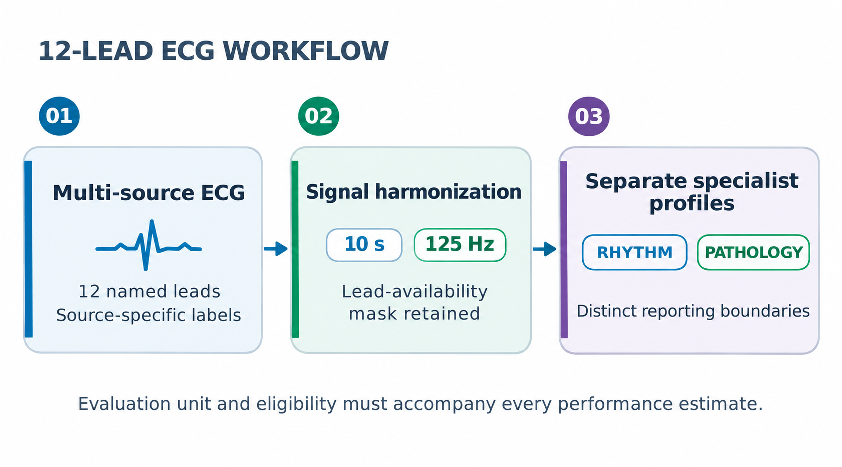
\includegraphics[width=\linewidth,height=.58\textheight,keepaspectratio]{fig00_ecg_ai_context}
\caption{Multi-source 12-lead ECG workflow mapping. The diagram displays the sequential transition from heterogeneous raw inputs to the separated rhythm and pathology specialist boundaries, illustrating the required physical harmonization constraints.\label{fig:fig00_ecg_ai_context}}
\end{figure}

\begin{figure}[htbp]
\centering
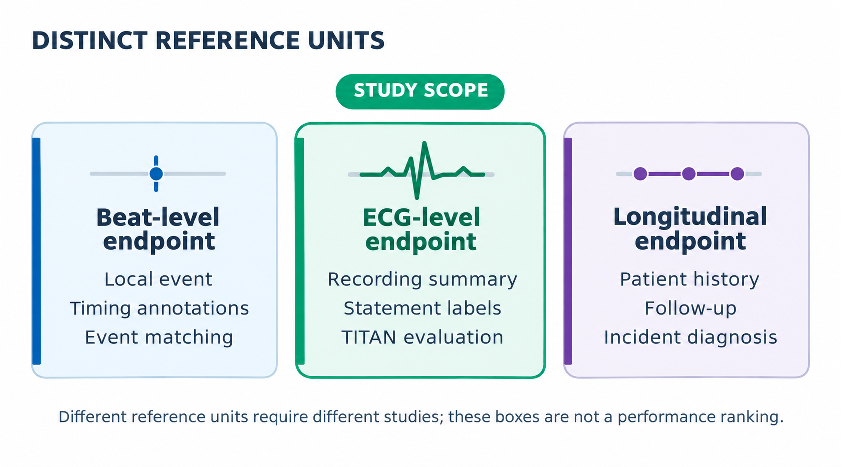
\includegraphics[width=\linewidth,height=.58\textheight,keepaspectratio]{fig00b_ecg_ai_evolution_gap}
\caption{Conceptual comparison of beat, ECG and longitudinal reference units. The study evaluates ECG-level statements only.\label{fig:fig00b_ecg_ai_evolution_gap}}

\end{figure}

\subsection{State of the Art and Comparative Literature}


Single-lead ambulatory classification and 12-lead statement classification are distinct tasks \citep{Hannun2019Cardiologist,Ribeiro2020Automatic}. PTB-XL and the PhysioNet Challenge make label and population differences explicit \citep{Wagner2020PTBXL,Strodthoff2021Deep,Reyna2022Challenge}. A dual-view CNN--Transformer has combined within-beat and recording-scale information \citep{Li2024DualView}. Other studies illustrate heterogeneous alternatives: uncertainty assessment on ECGs \citep{Vranken2021Uncertainty}, evaluation against expert consensus \citep{Herman2024}, and beat-level feature extraction and classification \citep{Mastoi2022DERMA,Elsheikhy2025Lightweight,Zhou2025Classification}. Their results cannot be placed on the same scale as the selected TITAN ECG and panel endpoints.

Table~\ref{tab:comparison} is a purposive comparison, not a systematic review or ranking. Direct ECG-AI comparators are studies sharing a multi-lead ECG input or related ECG statement outputs; beat-level and clinical workflow studies provide context only. Venue was not a selection criterion. NR denotes not reported or not comparable on the cited basis. Differences in labels, population, unit of analysis and validation design prevent direct ranking by published scores.

\begin{table}[htbp]
\caption{Selected ECG-AI studies across venues, compared by input, task and evaluation unit. The present study is intentionally excluded from this state-of-the-art table.\label{tab:comparison}}
\centering
\footnotesize
\begin{tabular}{@{}p{0.17\textwidth}p{0.25\textwidth}p{0.20\textwidth}p{0.28\textwidth}@{}}
\toprule
\textbf{Study / venue} & \textbf{Scope} & \textbf{Architecture / parameter reporting} & \textbf{Outputs and endpoint role} \\
\midrule
Mastoi et al. (2022), Life & ECG heartbeat classification with DERMA fusion & DERMA and FrIFT; SVM or KNN & Heartbeat rhythm-label task; Life ECG-AI comparator, not equivalent to 12-lead rhythm-plus-pathology specialist reporting \\
Ribeiro et al. (2020) & Large 12-lead diagnostic-abnormality classifier & Residual DNN; comparable params NR & Six diagnostic abnormalities; direct 12-lead comparator with different label scope and no cascade contract \\
Zhu et al. (2020) & Multi-label rhythm and conduction diagnosis & DNN; comparable params NR & Multi-label rhythm/conduction outputs; direct ECG-AI comparator with different ontology and no pathology specialist \\
Strodthoff et al. (2021) & PTB-XL benchmark across ECG deep learning models & Varies by benchmark model & SCP-style multi-label outputs; benchmark reference rather than one matched specialist architecture \\
Vranken et al. (2021) & Uncertainty-aware 12-lead ECG analysis & DNN; comparable params NR & 12-lead interpretation with uncertainty review; relevant to audit and uncertainty reporting \\
Herman et al. (2024) & Clinical validation of automated 12-lead interpretation & Proprietary; params NR & Broad ECG statements; clinical validation context rather than transparent architecture-size comparator \\
Li et al. (2024) & ECG abnormality classification & Dual-view CNN--Transformer & Beat and recording-scale information; distinct targets \\
Elsheikhy et al. (2025), MDPI & Beat classification in MIT-BIH and INCART & CNN with channel attention & Five beat classes, not P6/P4 \\
Zhou et al. (2025) & Multi-lead ECG classification with hierarchical features & Hierarchical CNN; comparable params NR & Beat classification on MIT-BIH and CCDD; not an ECG-level clinical cascade \\
\bottomrule
\end{tabular}
\end{table}


The objective was to design a modular 12-lead ECG classifier, characterize its specialist input and output contracts, and quantify accuracy, per-class discrimination and calibration on explicitly defined retrospective populations. The analysis separates evaluation of the released reporting profiles from later experiments addressing denominator sensitivity, morphology and selective prediction.

\section{Materials and Methods}

\subsection{Study Design and Evidence Boundary}


\label{sec:boundary}
This study designed and evaluated CNN--Transformer specialists on standardized ECG windows. The original release identifier \texttt{external\_dev}, termed external-development in the submission, refers to the archived selected development evaluations, not a single untouched test set. V3H used its 2,193-ECG P8 holdout for development validation; the selected P6 profile comprises 1,643 ECGs and its epoch selection used the reported P6 population. P4 uses four selected binary panels; 962 panel observations correspond to 733 unique ECGs, not 962 distinct patients. The panels are not all evaluated for every ECG. Table~\ref{tab:presentstudy} defines the profiles, and Table~\ref{tab:challengeposition} separates reporting choices from clinical decisions.

Independent external evaluation is a separate, unfinished analysis. Its intended confirmatory design binds cohort eligibility, source and patient/signal overlap checks, label mappings, frozen checkpoint bytes, preprocessing, thresholds and analysis endpoints before outcome review. Cohorts inspected during model selection, threshold fitting or domain adaptation are not counted as independent. Any unresolved overlap or reference incompatibility must be reported rather than assumed absent. No performance estimate from the ongoing independent evaluation is presented.
\begin{table}[htbp]
\caption{Present specialist evidence package reported in this manuscript.\label{tab:presentstudy}}
\centering
\scriptsize
\resizebox{\textwidth}{!}{%
\begin{tabular}{p{0.15\textwidth}p{0.23\textwidth}p{0.15\textwidth}p{0.29\textwidth}p{0.20\textwidth}}
\toprule
\textbf{Component} & \textbf{Role} & \textbf{Size/date} & \textbf{Output contract} & \textbf{Reported evidence} \\
\midrule
Backbone & Shared 12-lead CNN--Transformer representation & 58,352,219 & Common representation for rhythm, pathology, and auxiliary heads & Not used alone as a final clinical claim \\
Rhythm specialist & Selected Primary6 top-1 and binary membership & 63,930,847 & AFIB, SB, STACH, RBBB, 1AVB, PVC; cascade: NSR, PAC, flutter, paced & 95.19\% accuracy; 80.09\% macro-F1 \\
Pathology specialist & Selected Primary4 binary panels & 65,694,183 & ASMI, LVH, IMI, ISC\_; cascade: ALMI, ILMI; auxiliary: LAE & 80.23\% mean accuracy; 79.35\% macro-F1 \\
Evidence boundary & Frozen manuscript package & 2026-06-29 & Tables, figures, thresholds, source summaries, record probabilities, and hashes & Supports selected-result calculation; not historical replay \\
\bottomrule
\end{tabular}
}
\end{table}
\begin{table}[htbp]
\caption{Key challenges in multi-source ECG-AI reporting and the corresponding response in the present manuscript.\label{tab:challengeposition}}
\centering
\scriptsize
\resizebox{\textwidth}{!}{%
\begin{tabular}{p{0.18\textwidth}p{0.30\textwidth}p{0.32\textwidth}p{0.20\textwidth}}
\toprule
\textbf{Challenge} & \textbf{Why it matters} & \textbf{Study response} & \textbf{Where addressed} \\
\midrule
Heterogeneous ECG sources & Sampling rates, acquisition devices, countries, and annotation policies differ across public databases. & Keep source identity, harmonize to a fixed 10 s 12-lead contract, and report source-stratified selected development results. & Data curation, source audit, and Results source-stratified plots \\
Flat label compression & Rhythm, conduction, ischemia, infarction, and hypertrophy endpoints can be mixed into one output surface. & Separate Primary6 rhythm, Primary4 pathology, and unreported outputs. & Class-contract tables and specialist figures \\
Hidden minority-class behavior & High pooled accuracy can hide low recall or low F1 for clinically relevant minority labels. & Use macro-F1, classwise panels, row-normalized confusion matrices, ROC/PR curves, and balanced one-vs.-rest pathology panels. & Results tables, confusion matrices, and PR/ROC figures \\
Uncertain predictions & Low-margin or high-entropy cases may appear as hard labels unless review signals are preserved. & Distinguish score uncertainty, top-1, and explicitly tested withholding. & Uncertainty, calibration, and Grad-CAM sections \\
\bottomrule
\end{tabular}
}
\end{table}

\begin{figure}[htbp]
\centering
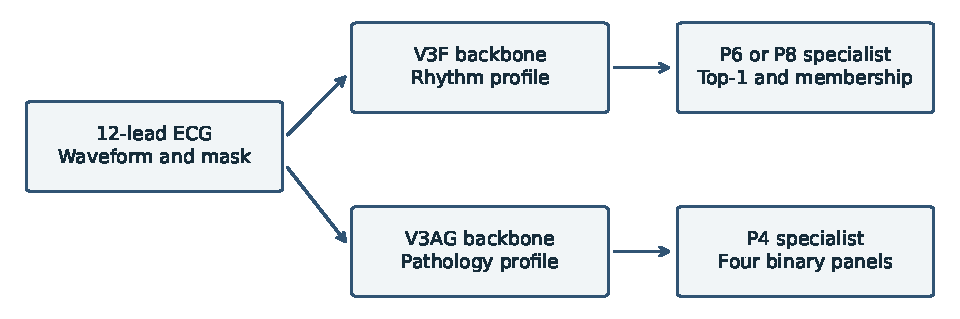
\includegraphics[width=\linewidth,height=.58\textheight,keepaspectratio]{fig01_graphical_abstract}
\caption{Specialist design. The P6/P8 and P4 evaluations use different fitted versions of the backbone design, V3F and V3AG, respectively.\label{fig:fig01_graphical_abstract}}

\end{figure}


Figure~\ref{fig:fig02_data_processing_bias_workflow} separates the reconstructed preprocessing steps from the provenance of the historical selected profiles and the unfinished independent assessment. Harmonizing waveform dimensions does not harmonize source annotation standards or demonstrate patient isolation.

\begin{figure}[htbp]
\centering
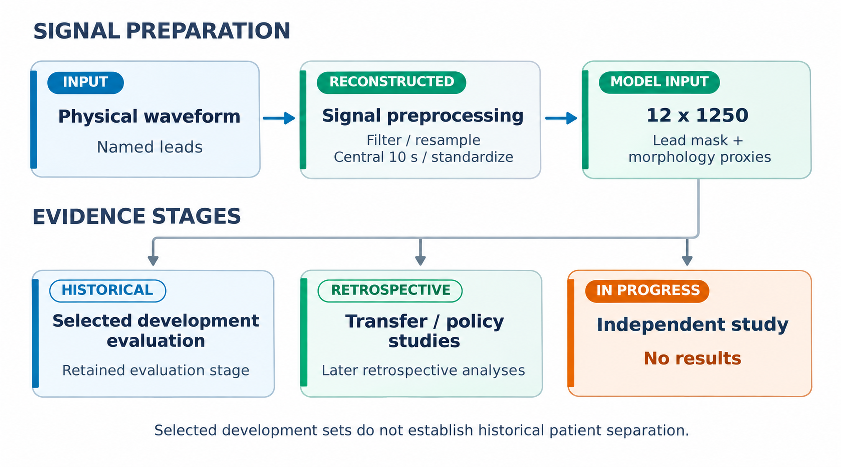
\includegraphics[width=\linewidth,height=.58\textheight,keepaspectratio]{fig02_data_processing_bias_workflow}
\caption{Signal preprocessing and distinct evidence stages. Selected development sets do not establish historical patient separation.\label{fig:fig02_data_processing_bias_workflow}}

\end{figure}


\subsubsection{Rationale for profile-specific reporting}
NSR is a physiologic rhythm and may be frequent in unselected populations. Its omission from P6 defines a narrower classification problem; it does not correct selection bias or establish a method for separating normal from abnormal ECGs. Similarly, the four P4 panels test specified statements, not every infarct territory or all structural disease. The role table distinguishes evaluation eligibility from proposed handling outside the profile.

\subsection{Dataset Curation, Harmonization, and Population-Shift Control}


\label{sec:data}
Separating patients and waveform duplicates is important because multiple ECGs or windows from one patient can share distinctive morphology. We distinguish source aliases, record-level exclusion and demonstrated patient/signal independence. The exact historical data loader and job-consumed train, calibration and validation rosters are not available for all checkpoints. The historical counts and the verified retrospective preprocessing are therefore reported separately below.

Throughout this mathematical formulation, scalar quantities ($f_s$, $T$, $z_{i,c}$) appear in standard italicized font, whereas column vectors ($\mathbf{x}_{i,\ell} \in \mathbb{R}^T$) and two-dimensional feature matrices ($\mathbf{X}_i \in \mathbb{R}^{L \times T}$) are distinguished by bold lowercase and uppercase notation, respectively. The standard twelve-lead spatial manifold follows the anatomical and projection sequence $\mathcal{L}=\{\mathrm{I},\mathrm{II},\mathrm{III},\mathrm{aVR},\mathrm{aVL},\mathrm{aVF},\mathrm{V1},\mathrm{V2},\mathrm{V3},\mathrm{V4},\mathrm{V5},\mathrm{V6}\}$, capturing frontal plane projections via the limb electrodes alongside horizontal planar views from the precordial montage. An unstandardized bioelectrical acquisition originating from source institution $i$ is formalized as:
\begin{equation}
\mathbf{R}_i \in \mathbb{R}^{L_i \times T_i^{\mathrm{raw}}}, \qquad f_i^{\mathrm{raw}}>0,
\end{equation}
where $L_i \le 12$ represents the quantity of active recording leads, $T_i^{\mathrm{raw}}$ denotes the native discrete temporal length, and $f_i^{\mathrm{raw}}$ characterizes the device-specific analog-to-digital sampling frequency.

Because multi-center clinical datasets inherently incorporate diverse acquisition hardware, varying analog filter topologies, and heterogeneous sampling protocols, inputs must undergo invariant temporal and topological transformation prior to tensor ingestion. To bridge this structural disparity, an invariant temporal resampling and lead-alignment operator $\mathcal{R}_{f_i^{\mathrm{raw}}\rightarrow f_s}$ is formulated to standardize disparate inputs:
\begin{equation}
\mathbf{X}_i=\mathcal{R}_{f_i^{\mathrm{raw}}\rightarrow f_s}\!\left(\mathbf{R}_i,\mathcal{L},10~\mathrm{s}\right), \qquad \mathbf{X}_i\in\mathbb{R}^{12\times1250},\quad f_s=125~\mathrm{Hz}.
\end{equation}

The tensor contract uses 125 Hz and ten seconds. Signal resampling and named-lead alignment are distinct from inference over the label ontology. A lead-validity mask is passed to the model separately from waveform values. This representation does not guarantee preservation of every high-frequency diagnostic feature or reconstruction of absent leads.

Inter-electrode contact impedance, patient respiration, and diverse amplifier calibration gains frequently superimpose low-frequency baseline fluctuations and scale discrepancies across multi-center recordings. To neutralize these confounding amplitude variations while preserving the diagnostic voltage ratios between adjacent cardiac complexes, dynamic lead-wise z-score standardization is executed independently across each temporal analysis window:
\begin{equation}
\tilde{\mathbf{x}}_{i,\ell}=\frac{\mathbf{x}_{i,\ell}-\mu_{i,\ell}\mathbf{1}}{\sigma_{i,\ell}+\epsilon}, \qquad \ell\in\mathcal{L},
\end{equation}
where $\mu_{i,\ell}$ and $\sigma_{i,\ell}$ signify the sample mean and empirical standard deviation computed exclusively across the temporal samples of lead $\ell$ within the active window, with $\epsilon = 10^{-8}$ incorporated to ensure numerical stability during near-isoelectric intervals. By determining normalization statistics strictly within the local temporal window of each specific tracing, this formulation avoids estimating a global normalization constant from pooled partitions; it does not prevent patient or signal overlap.

For extended diagnostic recordings from which multiple overlapping or sequential sliding windows $W_i$ are sampled, the architecture prevents overcounting biases during patient-level validation by aggregating predictions prior to nonlinear activation. The window-level uncalibrated logit vectors $z_{i,w,c}$ for class $c$ are averaged linearly across all constituent windows before applying the logistic sigmoid mapping:
\begin{equation}
z_{i,c}=\frac{1}{W_i}\sum_{w=1}^{W_i} z_{i,w,c},\qquad p_{i,c}=\sigma(z_{i,c}),
\end{equation}
This illustrates record-level pooling before activation. It prevents counting each window as a separate ECG in this score, but does not convert ECG counts into patient counts. The released profiles use their documented score and activation paths.

\subsubsection{Historical development populations and partitions}
\label{sec:history}

Files, windows, ECGs, patients and binary evaluation opportunities are distinct units. V3C records 9,021 training and 924 validation windows and removal of 390 record matches in its development roster. Job 16768 records 7,485 enumerated files and 9,945 windows: 9,021 train and 924 validation. The V3F reports separately record 9,021 rhythm training and 144 rhythm validation windows, and 5,013 pathology training and 776 pathology validation windows. These task-specific counts cannot be summed to count patients. The separate V3M/V3AG record-based split lists 9,885 training and 1,132 validation windows. P4 calibration job 17296 records 1,492 window--panel observations. Its exact roster and separation from all prior development stages were not authenticated.

PTB-XL, Chapman--Shaoxing, Ningbo, CPSC2018, CPSC2018-Extra, Georgia and CODE test appear among the retained aliases; a mixed local grouping is not a separate institution. Appendix~\ref{appendix:supplement} reports recoverable P6 and P4 source counts. Chapman--Shaoxing contributes 1,514 of 1,643 P6 ECGs. The joint training and validation table by source, class, window and patient cannot be recovered. A conditional metadata reconstruction for V3M/V3AG flagged possible shared patients despite distinct record identifiers. It neither identifies the bytes consumed by historical jobs nor demonstrates contamination of PTB-XL fold 10.

\subsubsection{ECG-associated reference statements}
\label{sec:af-reference}

For retained Challenge-format rows, atrial fibrillation (AF) and normal sinus rhythm (NSR) correspond to SNOMED CT codes 164889003 and 426783006. CPSC, Georgia, Chapman--Shaoxing and Ningbo rows use source-associated diagnosis fields, not a newly adjudicated reference. PTB-XL uses source Standard Communications Protocol for Computer-Assisted Electrocardiography (SCP-ECG) metadata, with mapped codes in its Challenge representation. CODE test uses supplied references; the mixed local group cannot be assumed to have a uniform annotation process. Source procedures differ and the archive does not authenticate all individual readers \citep{Reyna2022Challenge,Wagner2020PTBXL}.

Coexisting eligible labels are kept in the accepted reference set. Top-1 is correct if its class belongs to that set. One record contains both AF and NSR. P8 retains both and P6 excludes NSR by profile definition, not by adjudication. The AF code and retained reference agree in all 1,643 P6 and 2,193 P8 rows. Each overlapping profile has 390 AF-positive rows (373 Chapman--Shaoxing, 13 mixed local, four PTB-XL Challenge); the counts cannot be added. Other aliases have no AF-positive reference in these selected records, which does not estimate parent prevalence.

P4 references are panel-specific SCP-derived statements. The recorded label agrees with the relevant SCP key in 962/962 panel observations. This is mapping concordance, not an independent ECG reading or clinical adjudication. AF recognition is ECG-associated statement prediction, not detection of first diagnosis or incident disease, which requires longitudinal evidence \citep{Rossi2026AF}.


\subsection{Architecture and Specialist Branches}


Convolution and attention operate at different temporal scales. The former builds local waveform features, while the latter integrates information across the ten-second window. The description below summarizes the model design; the observed tensor widths and branch connectivity are reported separately.

Formally, let $\mathbf{X}_i \in \mathbb{R}^{12 \times 1250}$ represent the harmonized multi-lead input matrix. As the signal propagates through the convolutional feature extractor, the intermediate representation entering residual stage $b$, denoted by tensor $\mathbf{H}_b \in \mathbb{R}^{C_b \times T_b}$, is mapped to an upgraded subspace $\mathbf{H}_{b+1} \in \mathbb{R}^{C_{b+1} \times T_{b+1}}$ according to the residual formulation:
\begin{equation}
\mathbf{H}_{b+1}=\phi\!\left(F_b(\mathbf{H}_b;\boldsymbol{\theta}_b)+P_b(\mathbf{H}_b)\right),
\end{equation}
where the non-linear composite operator $F_b(\cdot;\boldsymbol{\theta}_b)$ embodies sequential one-dimensional convolutions, batch normalization layers, and dropout regularization parameterized by weight tensors $\boldsymbol{\theta}_b$. The operator $P_b(\cdot)$ denotes an identity or linear $1 \times 1$ projection shortcut designed to preserve uninterrupted gradient propagation across deep layer hierarchies, and $\phi(\cdot)$ specifies the Rectified Linear Unit ($\mathrm{ReLU}$) activation function \citep{He2016Deep}. This convolutional stem acts as an adaptive, multi-channel temporal filter bank that distills high-frequency morphological deflections directly from raw temporal traces.

Because standard 12-lead acquisitions project cardiac dipoles onto distinct anatomical planes, diagnostic information is inherently non-uniform across channels; for instance, anterior myocardial necrosis alters precordial leads V1--V4, whereas inferior ischemia manifests predominantly in leads II, III, and aVF. To dynamically prioritize informative spatial projections while suppressing noise-corrupted channels, a Squeeze-and-Excitation channel attention mechanism computes a recalibration vector $\mathbf{s} \in (0,1)^C$ from the post-residual feature representation $\mathbf{U} \in \mathbb{R}^{C \times T'}$ \citep{Hu2018Squeeze}:
\begin{equation}
\mathbf{s}=\sigma\!\left(\mathbf{W}_2\,\mathrm{SiLU}(\mathbf{W}_1\,\mathrm{GAP}(\mathbf{U}))\right),\qquad \widehat{\mathbf{U}}=\mathbf{s}\odot\mathbf{U},
\end{equation}
wherein $\mathrm{GAP}(\cdot)$ designates global average pooling executed across the discrete temporal dimension, contracting temporal activations into channel-wise summary statistics. The linear transformation matrices $\mathbf{W}_1$ and $\mathbf{W}_2$ form an excitation bottleneck, activated via the smooth Sigmoid Linear Unit ($\mathrm{SiLU}$), and $\sigma(\cdot)$ denotes the logistic sigmoid gate that scales the channel modulation vector $\mathbf{s}$. The element-wise Hadamard product $\odot$ produces the recalibrated tensor $\widehat{\mathbf{U}}$, dynamically amplifying clinically salient lead representations.

To capture non-local temporal patterns across multiple cardiac cycles, the recalibrated representations are processed by a multi-head scaled dot-product self-attention Transformer encoder \citep{Vaswani2017Attention}. This module models contextual interactions across arbitrary temporal distances within the tracing, formalizing attention weights as:
\begin{equation}
\mathrm{Attention}(\mathbf{Q},\mathbf{K},\mathbf{V})=\mathrm{softmax}\!\left(\frac{\mathbf{Q}\mathbf{K}^{\top}}{\sqrt{d_k}}\right)\mathbf{V},
\end{equation}
where $\mathbf{Q}$, $\mathbf{K}$, and $\mathbf{V}$ represent the projected query, key, and value matrices derived from the latent sequence, and the denominator $\sqrt{d_k}$ serves as a variance-stabilizing scaling factor to prevent gradient saturation in large inner-product regimes. The Transformer architecture is configured with 10 parallel self-attention heads operating over a latent model embedding dimension of $d_{\mathrm{model}}=640$, coupled to a position-wise feed-forward expansion layer of dimension $d_{\mathrm{ff}}=2560$.

The complete computational allocation and topological routing mechanisms are documented in Table~\ref{tab:architecture} and Table~\ref{tab:contracts}. Each loaded CNN--Transformer backbone object contains 58,352,219 parameters including its global heads. The rhythm package and pathology package comprise 63,930,847 and 65,694,183 parameters, respectively, including their separate fitted backbones. Reconstructed tensor interconnectivity and reporting roles are illustrated in Figure~\ref{fig:fig03_internal_architecture} and Figure~\ref{fig:fig03_cascade_contract}.

\begin{table}[htbp]
\caption{Architecture and parameter-count summary.\label{tab:architecture}}
\centering
\small
\resizebox{\textwidth}{!}{%
\begin{tabular}{lp{0.42\textwidth}rp{0.28\textwidth}}
\toprule
\textbf{Module} & \textbf{Description} & \textbf{Parameters} & \textbf{Scope} \\
\midrule
Input & 12-lead ECG & - & 12 x 1250 at 125 Hz \\
Shared backbone & ResNet-1D + Transformer + auxiliary heads & 58,352,219 & Separate multi-head representation \\
Rhythm package & Backbone + classwise rhythm specialist & 63,930,847 & Primary6 operational branch \\
Pathology package & Backbone + 512-unit pathology specialist & 65,694,183 & Primary4 operational branch \\
\bottomrule
\end{tabular}
}
\vspace{1ex}
\raggedright \footnotesize \textit{Note:} Total package parameters reflect the sum of the shared backbone, global attention heads, and the respective specialist branch.
\end{table}

\begin{table}[htbp]
\caption{Primary, secondary-candidate and auxiliary class contracts.\label{tab:contracts}}
\centering
\small
\begin{tabular}{llp{0.58\textwidth}}
\toprule
\textbf{Task} & \textbf{Role} & \textbf{Classes} \\
\midrule
Rhythm & Primary & AFIB, SB, STACH, RBBB, 1AVB, PVC \\
Rhythm & Secondary candidate & NSR, PAC, Flutter, Paced \\
Rhythm & Auxiliary global & LBBB, 2AVB, 3AVB, LQTS \\
Pathology & Primary & ASMI, LVH, IMI, ISC\_ \\
Pathology & Secondary candidate & ALMI, ILMI \\
Pathology & Auxiliary global & LAE \\
\bottomrule
\end{tabular}
\end{table}

\begin{figure}[htbp]
\centering
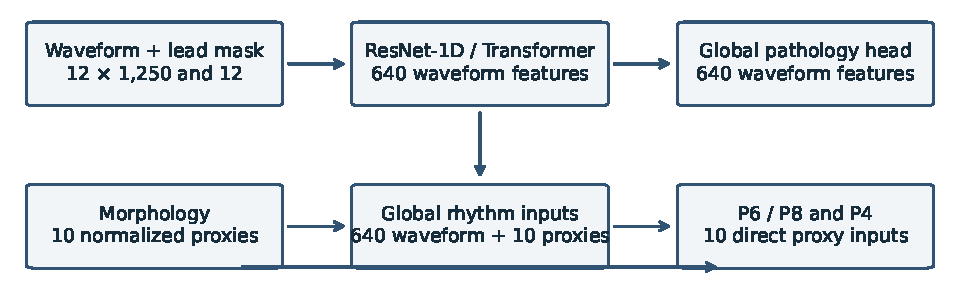
\includegraphics[width=\linewidth,height=.58\textheight,keepaspectratio]{fig03_internal_architecture}
\caption{Instrumented CNN--Transformer and specialist data flow. Arrows denote tensors passed in the reconstructed runtime. The ten morphology proxies feed both specialists directly; the global pathology head does not consume them directly.\label{fig:fig03_internal_architecture}}

\end{figure}

\begin{figure}[htbp]
\centering
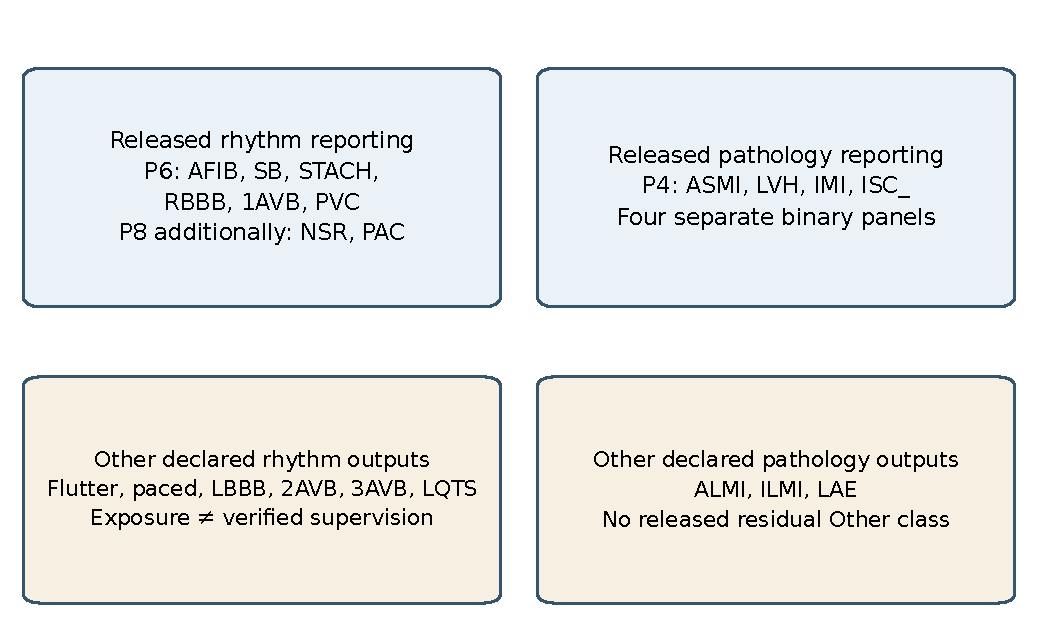
\includegraphics[width=\linewidth,height=.58\textheight,keepaspectratio]{fig03_cascade_contract}
\caption{Reporting and output contracts. Groupings do not describe a clinical dispatch rule and no arrow implies movement between groups.\label{fig:fig03_cascade_contract}}

\end{figure}

\subsubsection{Output definitions and direct supervision}
\label{sec:supervision}

Global rhythm and pathology heads expose 14 and seven outputs. P6 reports AFIB, sinus bradycardia (SB), sinus tachycardia (STACH), right bundle branch block (RBBB), first-degree atrioventricular block (1AVB), and premature ventricular contractions (PVC). P8 adds NSR and premature atrial contractions (PAC). P4 reports anteroseptal myocardial infarction (ASMI), left ventricular hypertrophy (LVH), inferior myocardial infarction (IMI), and ischemic ST--T change (ISC\_). V3F and V3AG are separate released backbone files. Shared design does not imply identical fitted weights.

Recovered V3F code indexes P8 in its rhythm loss (0.70 focal binary cross-entropy plus 0.30 categorical cross-entropy) and P4 in its pathology focal binary loss. Flutter, paced rhythm, left bundle branch block (LBBB), second- and third-degree atrioventricular block (2AVB and 3AVB), and long QT syndrome (LQTS) have no direct term in that V3F objective. Separate V3AG development code uses a different rhythm subset including Flutter and paced rhythm. Anterolateral and inferolateral myocardial infarction (ALMI and ILMI) and left atrial enlargement (LAE) are outside the recovered V3F direct pathology objective. This does not reconstruct earlier supervision or bind every runtime mask to released weights. Auxiliary metrics from 41M experiments cannot be attributed to V3F or V3AG. LQTS is not interchangeable with a prolonged-QT statement, nor is LAE automatically equivalent to left atrial overload (LAO).

In Table~\ref{tab:contracts}, \emph{Role} identifies a reporting or output contract. Primary outputs enter that profile's metrics; secondary candidates are outside the report and were proposed for separate handling; auxiliary endpoints are global outputs outside the specialist evaluation. These categories are not dispatch decisions. NSR is normal rhythm, excluded from P6 but included in P8. A residual Other group requires a specified ontology and reference; NSR should not be called Other arrhythmia.

\subsubsection{Reconstructed morphology inputs and tensor connections}
\label{sec:morphology}

The reconstruction used physical millivolt waveforms, a causal third-order Butterworth filter (0.5--45 Hz on nonconstant leads), polyphase resampling from 500 to 125 Hz, central ten seconds with padding when required, and per-lead standardization. The $12\times1250$ waveform has a 12-element lead mask. This contract was instrumented on LUDB, not authenticated as the exact historical loader.

The extractor uses lead II if nonflat, otherwise the highest-variance lead. Median-centered magnitude peaks exceed the larger of the 88th percentile and mean plus 0.8 standard deviations and are separated by at least 0.28 s. Positive inter-peak intervals $RR_i$ are in seconds. $E_{a:b}$ is one-sided Fourier power in the band, averaged across leads unless specified; $E_{\mathrm{tot}}$ is total power. Values are divided by the listed scales and clipped to $[0,1]$ (signed asymmetry $[-1,1]$); nonfinite values become zero.

\begin{table}[htbp]
\caption{Ten morphology descriptors. Width and pre-peak lag are proxies, not clinical intervals.\label{tab:morphology}}
\centering\small
\begin{tabular}{@{}p{.25\linewidth}p{.57\linewidth}p{.12\linewidth}@{}}
\toprule
Descriptor & Computation and unit & Scale \\
\midrule
Median heart rate & $60/\mathrm{median}(RR)$, beats/min & 220 \\
RR variation & Population $\mathrm{SD}(RR)/\mathrm{mean}(RR)$ & 1 \\
RMSSD & $10^3\sqrt{\mathrm{mean}[(RR_{i+1}-RR_i)^2]}$, ms & 500 \\
QRS-width proxy & Median span above max(35\% local maximum, 70th percentile) within 0.18 s of peak, ms & 220 \\
P-to-R proxy & Median lag to maximal pre-peak deflection 0.08--0.28 s before peak; retain lags 60--320 ms & 320 \\
QRS-band energy & $E_{5:18}/E_{\mathrm{tot}}$ & 1 \\
Low-frequency energy & $E_{0:0.7}/E_{\mathrm{tot}}$ & 1 \\
High-frequency energy & $E_{35:\mathrm{Nyq}}/E_{\mathrm{tot}}$ & 1 \\
Cross-lead correlation & Mean absolute off-diagonal Pearson correlation over nonflat leads & 1 \\
Limb-lead asymmetry & $(E_I-E_{aVF})/\max(E_I+E_{aVF},10^{-12})$ in 5--18 Hz & 1 \\
\bottomrule
\end{tabular}
\end{table}

The global rhythm head receives a 640-dimensional waveform/mask embedding and ten descriptors (width 650). The global pathology head receives the embedding without direct morphology. P6/P8 (681 inputs) and P4 (670 inputs) both receive morphology at indices 640--649 alongside task-specific score or event inputs. P4 also receives rhythm scores. Stored rhythm head width 512 supersedes stale metadata declaring 192; P4 hidden width is also 512. The 58,352,219-parameter backbone count includes the global heads, and does not describe the separate 41M models.

A flat-signal fixture produced spurious plateau peaks and nonzero descriptors. The proxies are not clinically validated. Job 33796 instrumented both tensor paths on 16 LUDB ECGs and exactly repeated a reconstructed fixed-batch forward. This is not historical waveform replay: a separate strict P4 comparison exceeded the score tolerance for 836/962 observations even though threshold decisions agreed in that comparison.

\subsubsection{Separate retrospective analyses}
\label{sec:retrospective-methods}

The Shanghai People's Hospital (SPH) analysis applied released profiles to all 25,770 metadata ECGs (24,666 source patient identifiers) before forming nested profile-compatible subsets from the same scores. Absence of a compatible statement is negative for the mapped endpoint, not adjudicated absence of disease. The primary SPH mapping does not supply 1AVB, NSR or ISC\_ references. A PTB-XL folds 1--9 development cache supplied separate 1AVB and ISC\_ statements; 6,205 of 19,601 metadata ECGs were technically scored. LUDB and PTB Diagnostic are separate sources and cannot replace SPH or the missing June population.

Other experiments fit new development heads. The rhythm residual covers mapped out-of-profile statements; normal rhythm and unknown references remain distinct. The pathology residual is a bounded PTB-XL ALMI/ILMI/LAO-or-LAE union. A morphology ablation fit equal-capacity heads with fixed backbone representations, five matched seeds per arm, and simultaneous intervals against a predefined $\pm2$ percentage-point relevance margin. These are not independent validation, full-network retraining, or changes to the released models.

\subsection{Loss Function, Optuna Search, Fine-Tuning, and Calibration}


\label{sec:optimization}
Class imbalance motivated a focal binary term \citep{Lin2017Focal}. For a known binary target $y_{ic}$, let $p_{t,ic}=p_{ic}$ when $y_{ic}=1$ and $p_{t,ic}=1-p_{ic}$ otherwise. With eligibility mask $m_{ic}$, the focal term is
\begin{equation}
\mathcal L_{\mathrm{focal}}=-\frac{\sum_{ic}m_{ic}\alpha_{ic}(1-p_{t,ic})^\gamma\log(p_{t,ic}+\epsilon)}{\sum_{ic}m_{ic}}.
\end{equation}
Here $\alpha_{ic}$ denotes a class/target weight when used. Masked or unrecognized labels do not contribute to the corresponding term. The categorical component uses $-\sum_c q_{ic}\log \mathrm{softmax}(z_i)_c$ for target vector $q_i$. The archived 50-epoch development run records auxiliary clinical-axis losses; it does not show that the released specialist decision has a validated auxiliary function. Exact historical configuration and label support are not available for all prior stages.

The V3C Optuna selection used a TPE sampler (recorded seed 197813, multivariate mode, ten startup trials), with 12 planned trials and nine retained completed candidates, distinct from V4 and the 41M screening series \citep{Akiba2019Optuna}. The recorded epoch composite was
\begin{equation}
J_e=0.6F1_{\mathrm{P8},e}+0.4F1_{\mathrm{P4},e}-0.05M_{\mathrm{P8},e}-0.05M_{\mathrm{P4},e},
\end{equation}
where $M$ denotes missing target classes or labels, not mini-batch variance. Candidate ranking uses the mean of the last three composites less 0.25 times their population standard deviation. Trial 6 led that ranking (0.624512); trial 8 had the highest single-epoch peak (0.650940). The selection JSON and archived effective configuration agree on the parameters in Table~\ref{tab:optuna}. Job 16768 ran 50 epochs; job 16781 subsequently declared its intermediate checkpoint as the initialization for V3F. The V3F report records eight epochs. The historical V3F output digest agrees with the published backbone. The original Optuna database, intermediate checkpoint bytes and job-level input/output digest binding remain unavailable; neither scheduler completion nor the output digest proves the complete byte-level lineage.

\begin{table}[htbp]
\caption{Recorded V3C trial 6 hyperparameters used in the archived job 16768 configuration.\label{tab:optuna}}
\centering
\small
\begin{tabular}{lr}
\toprule
\textbf{Parameter} & \textbf{Selected value} \\
\midrule
base\_lr & 6.5005e-06 \\
max\_lr & 9.7576e-05 \\
weight\_decay & 7.9107e-06 \\
gamma & 1.5254 \\
label\_smoothing \citep{Szegedy2016Rethinking} & 0.018121 \\
batch\_size & 16 \\
mixup\_alpha & 0.033822 \\
lambda\_pathology & 0.24551 \\
\bottomrule
\end{tabular}
\end{table}


\subsubsection{Thresholds, top-1 and empty prediction sets}
\label{sec:decision}
For a binary statement, the thresholded decision is $\hat y_{ic}=\mathbb{1}[p_{ic}\ge \tau_c]$. For rhythm, the released top-1 output is distinct from the membership set. P6 retains the top-1 label on every selected ECG even when the binary set is empty; empty membership remains all-negative in P6 binary metrics. P8 fills an empty predicted set with the recorded top-1 class. The top-1 correctness criterion is membership in the accepted reference set. P4 remains a binary panel evaluation: below threshold is negative and remains in the panel denominator. Thresholds are the released values in Tables~\ref{tab:rhythmclass}, \ref{tab:pathclass} and \ref{tab:p8class}. None of these cases is automatically a clinical abstention.

\subsection{Uncertainty and selective prediction}
\label{sec:selective}
Predictive entropy $H(p)=-\sum_c p_c\log p_c$ and the difference between the two highest probabilities can describe uncertainty for a categorical score. With $T$ stochastic passes, the difference between entropy of the mean probability and mean entropy is a model-dependent diagnostic; it is not proof of out-of-distribution status. The original June report has no authenticated decision ledger connecting these statistics to actual withholding, secondary inference or expert review. Historical quarantine rates and pre/post accuracy are therefore not reported.

In the later score-based P8/P4 experiment, profile confidence was the minimum absolute distance between class scores and the respective released cutoffs. The profile cutoffs (P8: 0.037162775; P4: 0.014417143) were fitted for target coverage on 12,901 SPH calibration ECGs without reference labels. The frozen joint rule emits both decisions only if both profile cutoffs are met. Failure to produce scores is distinct from abstention. With $N_s$ scored ECGs and $N_a$ accepted ECGs, coverage is $N_a/N_s$ and the scored abstention rate is $(N_s-N_a)/N_s$. Coverage relative to all enrolled ECGs is reported separately when some cannot be scored. Pre-policy risk is FP plus FN divided by known binary opportunities over all scored ECGs; post-policy risk uses only accepted opportunities. Withheld positives are separate from emitted false negatives. The full-denominator cost counts emitted errors plus $\lambda$ times withheld known opportunities. A separate LUDB experiment runs actual P6 fallback only on withheld ECGs, with frozen P6 membership thresholds, no top-1 override and no clinician review.

\subsection{Grad-CAM Explainability Contract}

Clinical adoption of deep learning models in electrophysiology requires rigorous algorithmic interpretability that confirms predictions are grounded in true electrophysiological wave morphology rather than spurious baseline noise or high-frequency acquisition artifacts. To satisfy this explainability requirement, the architecture implements class-discriminative one-dimensional Gradient-weighted Class Activation Mapping (1D Grad-CAM) \citep{Selvaraju2017Grad} coupled to a strict audit contract. For a targeted diagnostic class $c$ with pre-activation score $y^c$ and intermediate temporal activation tensor $A_k(t)$ in convolutional feature channel $k$, spatial-temporal importance weights $\alpha_k^c$ are computed by averaging gradients across the temporal length $T'$:
\begin{equation}
\alpha_k^c=\frac{1}{T'}\sum_{t=1}^{T'}\frac{\partial y^c}{\partial A_k(t)}.
\end{equation}
The resulting channel-weighted linear combination is passed through a Rectified Linear Unit activation to isolate strictly positive contributions toward the target class, producing the continuous temporal saliency profile:
\begin{equation}
L_{\mathrm{GradCAM}}^c(t)=\mathrm{ReLU}\left(\sum_k \alpha_k^c A_k(t)\right).
\end{equation}
The temporal heatmap indicates local gradient-weighted activation, not validated identification of an electrophysiological complex. This defines an explainability method and recommended metadata, not a validated explanation of decision causality or an inventory of all historical artifacts.

\subsection{Evaluation Metrics and Confidence Intervals}


\label{sec:metrics}
For each known binary opportunity, TP, TN, FP and FN count true positives, true negatives, false positives and false negatives. With $N=TP+TN+FP+FN$,
\begin{align}
\mathrm{Acc}_{\mathrm{bin}}&=(TP+TN)/N,&
\mathrm{PPV}=\mathrm{Precision}&=TP/(TP+FP),\\
\mathrm{Sensitivity}=\mathrm{Recall}&=TP/(TP+FN),&
\mathrm{Specificity}&=TN/(TN+FP),\\
\mathrm{NPV}&=TN/(TN+FN),&
F1&=2TP/(2TP+FP+FN).
\end{align}
Undefined denominators are not treated as clinical zeros. With $C$ class endpoints, $\mathrm{MacroF1}=C^{-1}\sum_c F1_c$; mean binary accuracy is $C^{-1}\sum_c\mathrm{Acc}_{\mathrm{bin},c}$. Top-1 accuracy is $n^{-1}\sum_i\mathbb{1}[\hat c_i\in S_i]$ for the accepted reference set $S_i$ and one emitted top-1 class $\hat c_i$. P6 top-1 and mean binary F1 use different decision units; P4 mean binary accuracy is not top-1 or pooled panel accuracy.

With $\mathrm{TPR}$ and $\mathrm{FPR}$ denoting the true- and false-positive rates, $\mathrm{AUROC}=\int_0^1\mathrm{TPR}\,d\mathrm{FPR}$ for the binary ranking curve \citep{Hanley1982meaning}. Average precision (AP) is $\sum_k (R_k-R_{k-1})P_k$ at successive distinct score thresholds, not trapezoidal PR area. Brier score is $n^{-1}\sum_i(p_i-y_i)^2$. For ten equally spaced probability bins, binary expected calibration error (ECE) is $\sum_b(n_b/n)|\bar p_b-\bar y_b|$ over nonempty bins. The vertical axis of the reliability plots is $\bar y_b$, the fraction of reference-positive observations in bin $b$.

The Wilson 95\% interval for $k/n=\hat p$ is
\begin{equation}
\frac{\hat p+z^2/(2n)\ \pm\ z\sqrt{\hat p(1-\hat p)/n+z^2/(4n^2)}}{1+z^2/n},\quad z=1.96.
\end{equation}
Selected-source Wilson intervals use ECGs as observations \citep{Wilson1927Probable}. Classwise F1 bars use the 2.5th and 97.5th percentiles of 1,000 row-level bootstrap draws from their observed binary confusion counts \citep{Efron1979Bootstrap}. These are descriptive within-panel intervals, not patient-level uncertainty. The later SPH studies report component intervals for their own contrasts.

\begin{table}[htbp]
\caption{Metric definitions used in the manuscript package.\label{tab:metrics}}
\centering
\small
\resizebox{\textwidth}{!}{%
\begin{tabular}{lp{0.55\textwidth}p{0.24\textwidth}}
\toprule
\textbf{Metric} & \textbf{Definition} & \textbf{Use} \\
\midrule
Top-1 accuracy & Correct primary class predictions divided by evaluated records & Multiclass rhythm \\
Mean binary accuracy & Arithmetic mean of one-vs.-rest class accuracies & Multilabel pathology \\
Macro-F1 & Unweighted mean of classwise F1 scores & Both tasks \\
AUROC & Area under the receiver operating characteristic curve & one-vs.-rest \\
Average precision & Recall-weighted precision at distinct score thresholds & one-vs.-rest \\
Brier score & Mean squared error between predicted probabilities and binary outcomes & Probability calibration \\
ECE & Ten-bin expected calibration error & Probability calibration \\
\bottomrule
\end{tabular}
}
\end{table}

\section{Results}

\subsection{Overall Specialist Performance}


Table~\ref{tab:overall} reports the selected development evaluations. P6 correctly assigned a top-1 class to 1,564 of 1,643 ECGs (95.19\%) and had thresholded mean binary F1 of 80.09\%. P4 had mean panel accuracy of 80.23\% and macro-F1 of 79.35\% across 962 ECG--label observations from 733 unique ECGs. The P8 development profile achieved 90.61\% top-1 and 76.14\% mean binary F1 across 2,193 ECGs. The profiles overlap and are not independent comparators. None estimates a clinical all-input workflow.

\begin{table}[htbp]
\caption{Selected development performance. Rhythm denominators count ECGs; P4 counts panel observations.\label{tab:overall}}
\centering
\small
\resizebox{\textwidth}{!}{%
\begin{tabular}{llrcccc}
\toprule
\textbf{Specialist} & \textbf{Contract} & \textbf{Observations} & \textbf{Primary Accuracy} & \textbf{Macro-F1} & \textbf{Macro-AUROC} & \textbf{Macro-AP} \\
\midrule
Rhythm & Primary6 multiclass (top-1) & 1,643 & 95.19\% & 80.09\% & 96.53\% & 85.61\% \\
Pathology & Primary4 one-vs.-rest panels & 962 & 80.23\% & 79.35\% & 87.46\% & 87.85\% \\
\bottomrule
\end{tabular}
}
\end{table}


Figure~\ref{fig:fig06_rhythm_confusion} reports top-1 classification for the 1,460 ECGs with exactly one accepted class. The overall top-1 denominator also includes 183 ECGs with more than one accepted class. Figure~\ref{fig:fig08_class_metrics} and Table~\ref{tab:rhythmclass} report thresholded binary precision, recall and F1 on all 1,643 ECGs, not the single-reference subset. The 1AVB F1 of 62.58\% and PVC F1 of 65.64\% indicate substantial residual errors; neither supports reliable clinical performance.

\begin{figure}[htbp]
\centering
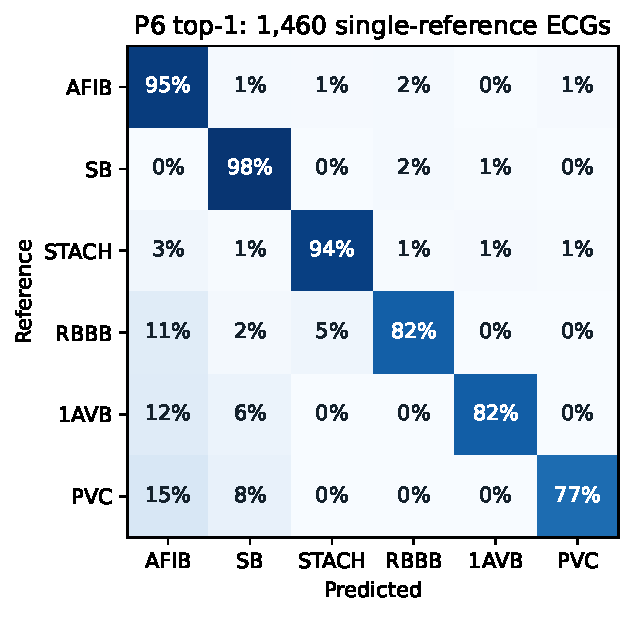
\includegraphics[width=\linewidth,height=.58\textheight,keepaspectratio]{fig06_rhythm_confusion}
\caption{Primary6 top-1 confusion on the 1,460 single-reference ECGs. Cells are row percentages.\label{fig:fig06_rhythm_confusion}}

\end{figure}

\begin{figure}[htbp]
\centering
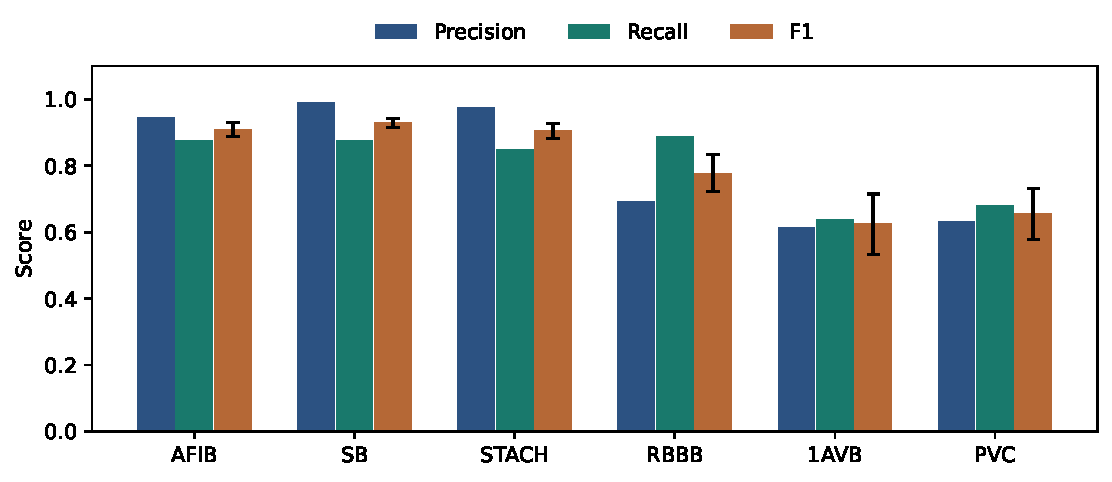
\includegraphics[width=\linewidth,height=.58\textheight,keepaspectratio]{fig08_class_metrics}
\caption{Primary6 classwise precision, recall and F1 on 1,643 ECGs. F1 bars include 95\% row-bootstrap intervals; the plotted quantities are classwise, not macro averages.\label{fig:fig08_class_metrics}}

\end{figure}

\begin{table}[tbp]
\caption{P6 statement-level decisions at the released thresholds. Positives are reference statements.\label{tab:rhythmclass}}
\centering\small
\begin{tabular}{lrrrrrrr}
\toprule
Class & Positive & Total & Precision & Recall & Specificity & F1 & Cutoff \\
\midrule
AFIB & 390 & 1643 & 94.48\% & 87.69\% & 98.40\% & 90.96\% & 0.820 \\
SB & 792 & 1643 & 99.14\% & 87.50\% & 99.29\% & 92.96\% & 0.835 \\
STACH & 362 & 1643 & 97.46\% & 84.81\% & 99.38\% & 90.69\% & 0.775 \\
RBBB & 116 & 1643 & 69.13\% & 88.79\% & 96.99\% & 77.74\% & 0.515 \\
1AVB & 80 & 1643 & 61.45\% & 63.75\% & 97.95\% & 62.58\% & 0.570 \\
PVC & 94 & 1643 & 63.37\% & 68.09\% & 97.61\% & 65.64\% & 0.430 \\
\bottomrule
\end{tabular}
\end{table}

\subsection{Pathology Primary4 Results}


Table~\ref{tab:pathclass} and Figures~\ref{fig:fig07_pathology_confusion} and \ref{fig:fig08b_pathology_class_metrics} report the four binary panels. ASMI, LVH, IMI and ISC\_ contribute 294, 224, 206 and 238 observations, respectively. One ECG may occur in multiple panels. ISC\_ had F1 of 91.56\%, compared with 65.73\% for LVH; this difference does not establish performance in unselected clinical patients.

\begin{table}[tbp]
\caption{P4 statement-level decisions at the released thresholds. Positives are reference statements.\label{tab:pathclass}}
\centering\small
\begin{tabular}{lrrrrrrr}
\toprule
Class & Positive & Total & Precision & Recall & Specificity & F1 & Cutoff \\
\midrule
ASMI & 147 & 294 & 92.98\% & 72.11\% & 94.56\% & 81.23\% & 0.670 \\
LVH & 112 & 224 & 69.31\% & 62.50\% & 72.32\% & 65.73\% & 0.705 \\
IMI & 103 & 206 & 76.36\% & 81.55\% & 74.76\% & 78.87\% & 0.635 \\
ISC\_ & 119 & 238 & 97.17\% & 86.55\% & 97.48\% & 91.56\% & 0.595 \\
\bottomrule
\end{tabular}
\end{table}

\begin{figure}[htbp]
\centering
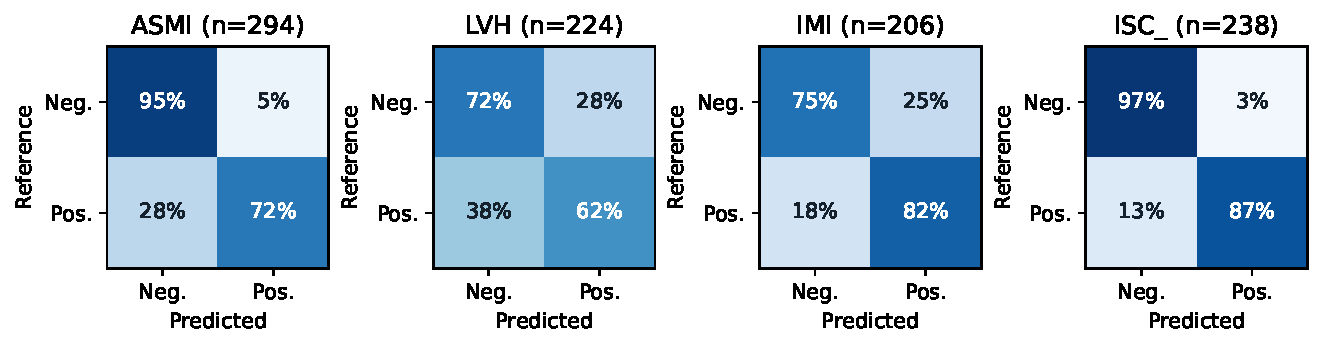
\includegraphics[width=\linewidth,height=.58\textheight,keepaspectratio]{fig07_pathology_confusion}
\caption{Primary4 confusion matrices for the four binary panels. Cells are row percentages; per-panel denominators are shown above each matrix.\label{fig:fig07_pathology_confusion}}

\end{figure}

\begin{figure}[htbp]
\centering

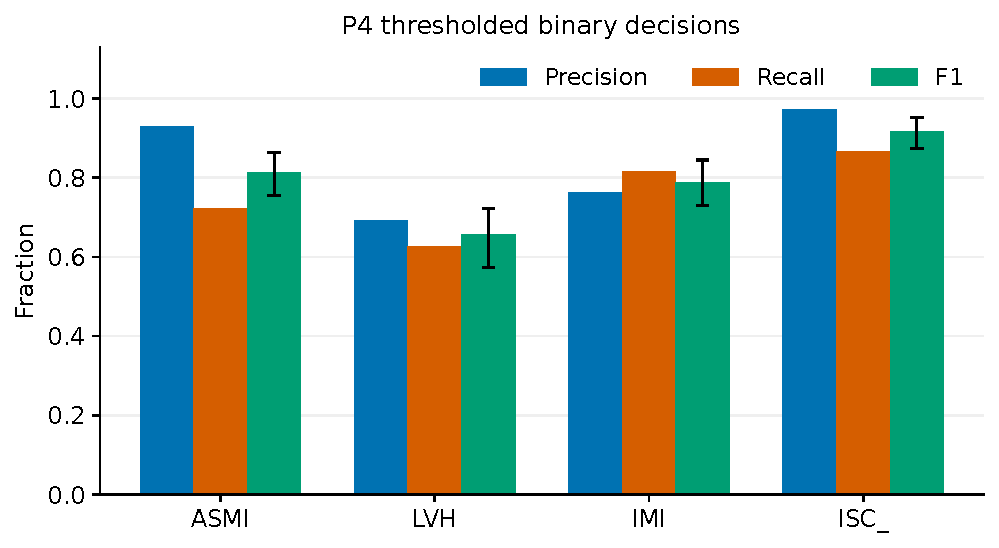
\includegraphics[width=\linewidth]{fig08b_pathology_class_metrics}
\caption{Primary4 classwise precision, recall and F1. F1 bars show 95\% row-bootstrap intervals. These four pathology panels are distinct from the six rhythm classes.\label{fig:fig08b_pathology_class_metrics}}

\end{figure}

\subsection{Discrimination, Calibration, and Uncertainty}


Figures~\ref{fig:fig09_roc_curves} and \ref{fig:fig10_precision_recall_curves} show classwise ranking for P6 ECGs and P4 panel observations. Macro-AUROC was 96.53\% and 87.46\%, respectively. The estimates refer to different selected tasks and neither establishes calibration or clinical discrimination in an unselected population. With average precision defined as the recall-weighted sum, macro-AP was 85.61\% and 87.85\%. Brier scores ranged from 0.024 (SB) to 0.042 (1AVB) in P6 and 0.078 (ISC\_) to 0.224 (LVH) in P4. Figure~\ref{fig:fig11_calibration} compares mean predicted probability with observed positive frequency in each populated bin.

\begin{figure}[htbp]
\centering
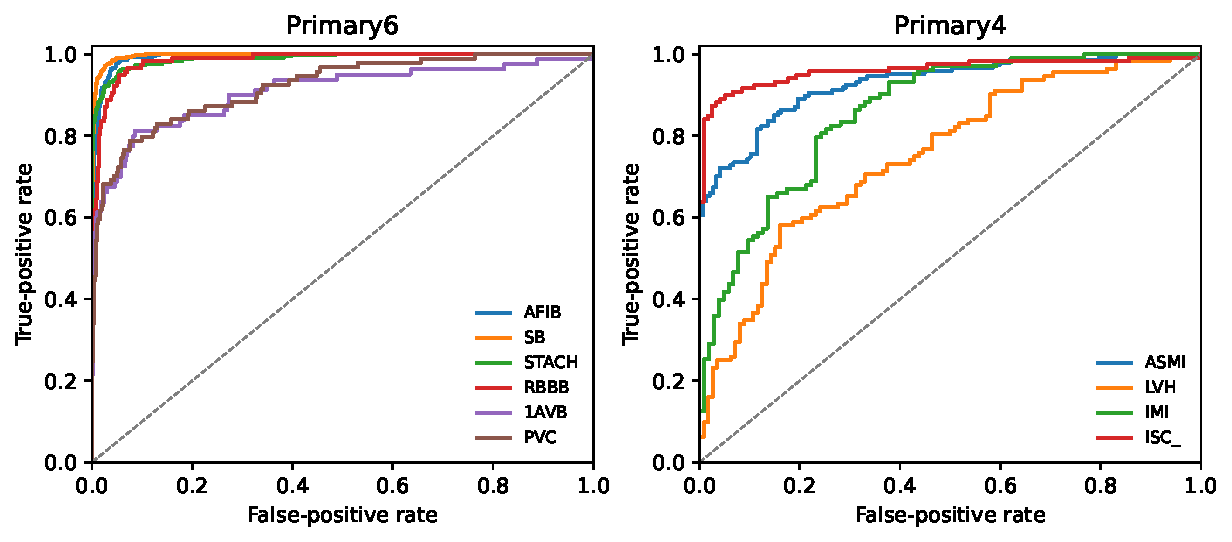
\includegraphics[width=\linewidth,height=.58\textheight,keepaspectratio]{fig09_roc_curves}
\caption{Receiver operating characteristic (ROC) curves. Classwise performance is mapped against the diagonal baseline for rhythm (left) and pathology (right).\label{fig:fig09_roc_curves}}
\end{figure}

\begin{figure}[htbp]
\centering
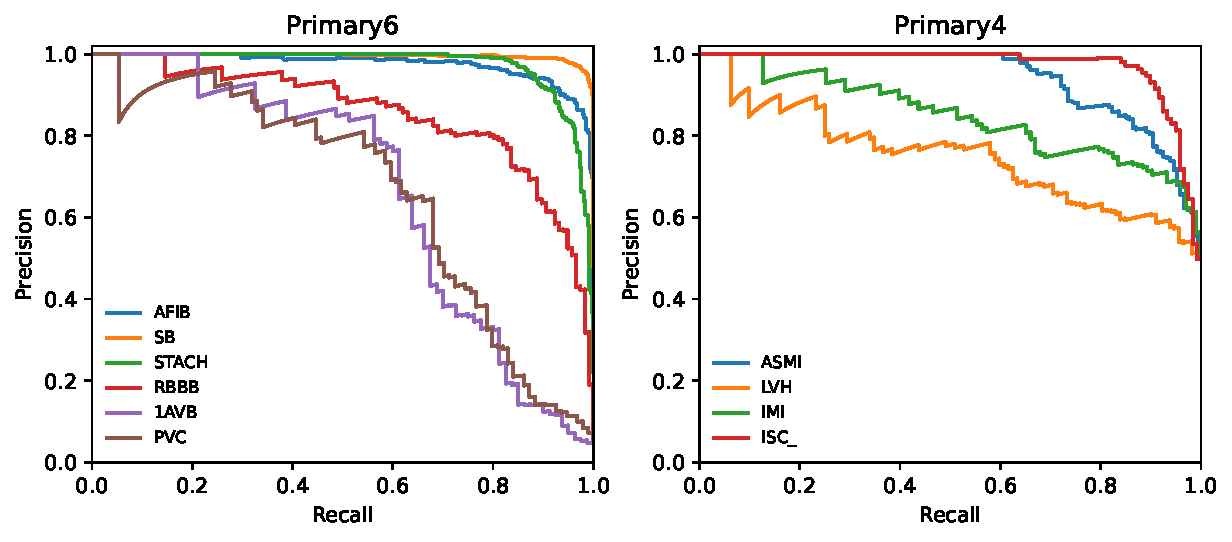
\includegraphics[width=\linewidth,height=.58\textheight,keepaspectratio]{fig10_precision_recall_curves}
\caption{Precision-recall (PR) curves for rhythm (left) and pathology (right) branches. Curves document ranking quality across varying operational decision thresholds.\label{fig:fig10_precision_recall_curves}}
\end{figure}

\begin{figure}[htbp]
\centering
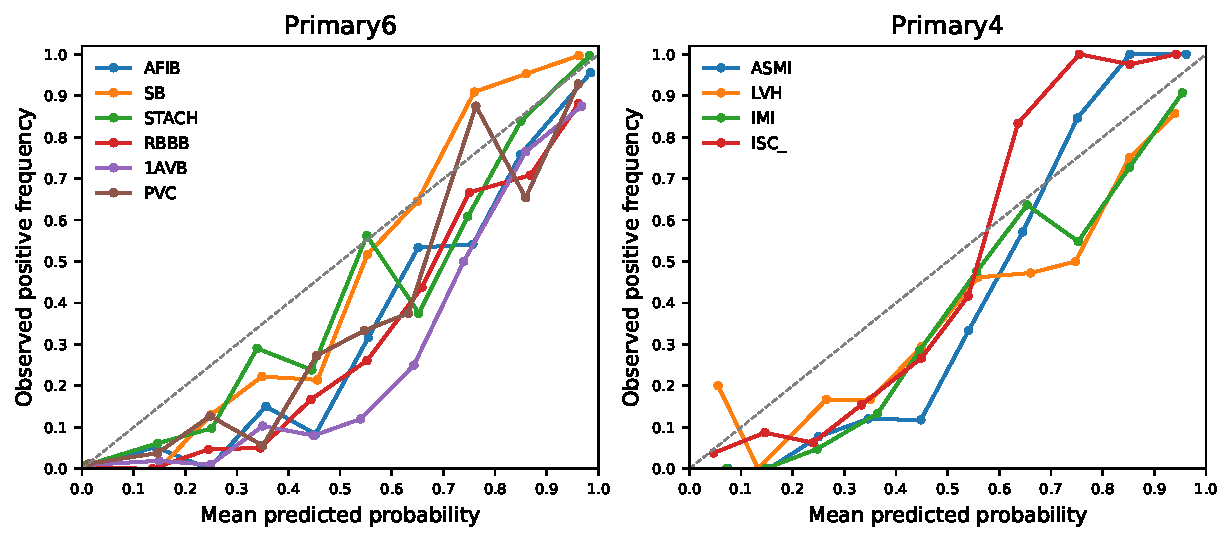
\includegraphics[width=\linewidth,height=.58\textheight,keepaspectratio]{fig11_calibration}
\caption{Reliability diagrams in ten equal-width probability bins. The vertical axis is the observed positive reference fraction; empty bins have no estimate.\label{fig:fig11_calibration}}

\end{figure}


Threshold-empty output counts are reported separately in Section~\ref{sec:selective-results}. No historical pre/post-quarantine estimate can be computed from the retained records.

\subsection{Source-Stratified Robustness and Error Analysis}


Figure~\ref{fig:fig12_source_performance} describes P6 top-1 accuracy by retained source alias. The support varies substantially: Chapman--Shaoxing contributes 1,514 ECGs, while five to 19 ECGs are represented in several other groups. The resulting Wilson intervals should not be interpreted as evidence of stable transport across institutions.

\begin{figure}[htbp]
\centering
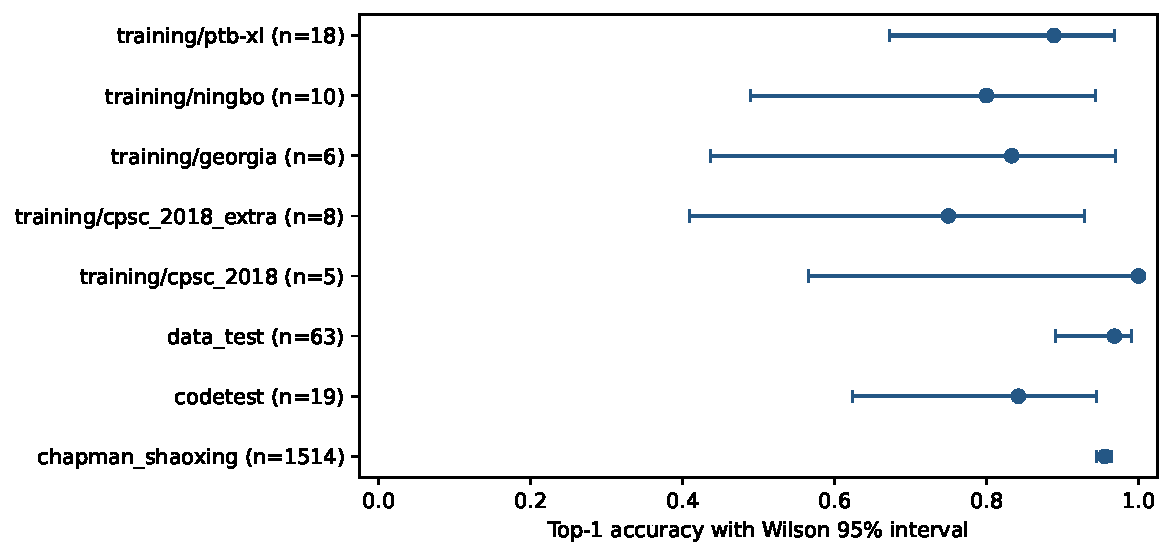
\includegraphics[width=\linewidth,height=.58\textheight,keepaspectratio]{fig12_source_performance}
\caption{Source-stratified Primary6 rhythm top-1 accuracy. Variations are grouped by origin dataset family, complete with Wilson score 95\% confidence intervals.\label{fig:fig12_source_performance}}
\end{figure}

\begin{figure}[htbp]
\centering
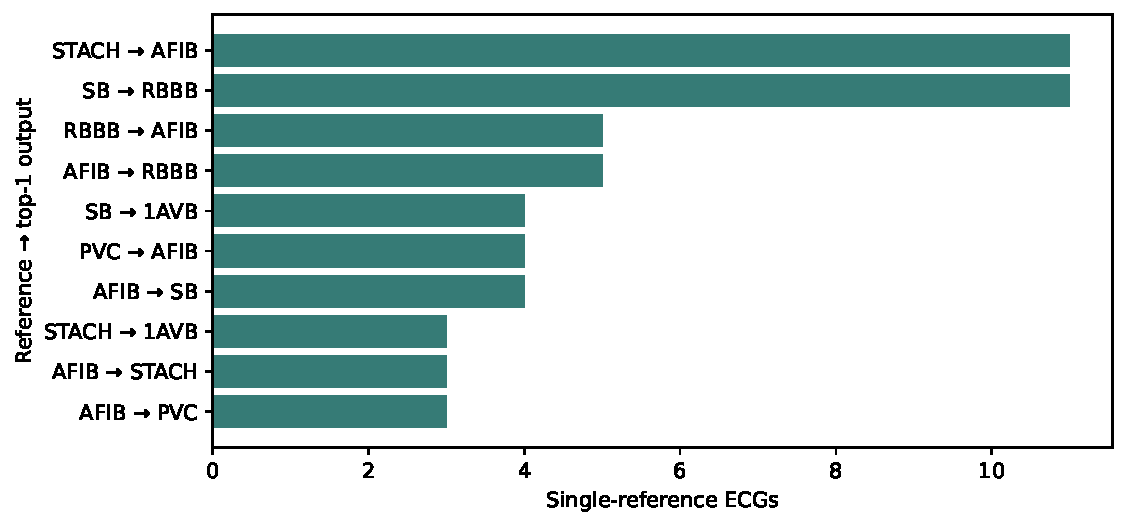
\includegraphics[width=\linewidth,height=.58\textheight,keepaspectratio]{fig13_error_flows}
\caption{Frequent P6 reference-to-top-1 errors in the single-reference subset. Bars count ECGs; no bar represents a quarantine or referral.\label{fig:fig13_error_flows}}

\end{figure}

\subsection{Denominator sensitivity in retrospective transfer}
\label{sec:transfer-results}

All 25,770 SPH ECGs were scored by each released profile in the all-input comparison. The unchanged scores gave mapped macro-F1 of 0.7083 (P6), 0.6622 (P8), and 0.0388 (P4) across the full cohort, compared with 0.9057, 0.8553, and 0.7278 in the nested profile-compatible subsets (5,523, 5,925, and 415 ECGs, respectively). These are averages over compatible statements, not the original P6 top-1 task or the P4 selected panel experiment. Different class prevalences and denominators change the interpretation. For example, the SPH PVC reference has 1,067 positive and 24,703 absent-statement comparisons; P6 PVC F1 was 54.08\% and P8 PVC F1 was 66.16\%. Table~\ref{tab:sph_endpoints} reports statement predictive values and patient-component F1 intervals on the original SPH denominator. These results do not supply the missing full June workflow or establish an independent confirmatory result.

\begin{table}[htbp]
\caption{Retrospective SPH full-denominator mapped endpoints. Each row contains 25,770 ECG statements. F1 intervals use 2,000 patient and duplicate component bootstrap draws. Unmapped endpoints are omitted.\label{tab:sph_endpoints}}
\centering\small
\begin{tabular}{lrrrrrr}
\toprule
Endpoint & Positive & PPV & Recall & NPV & F1 & F1 95\% CI \\
\midrule
P6:AFIB & 675 & 84.86\% & 93.04\% & 99.81\% & 88.76\% & 86.92\%--90.38\% \\
P6:SB & 2,711 & 68.41\% & 82.18\% & 97.85\% & 74.66\% & 73.46\%--75.83\% \\
P6:STACH & 725 & 77.06\% & 85.24\% & 99.57\% & 80.94\% & 78.62\%--83.08\% \\
P6:RBBB & 710 & 39.13\% & 96.62\% & 99.90\% & 55.70\% & 53.15\%--58.12\% \\
P6:PVC & 1,067 & 39.69\% & 84.82\% & 99.31\% & 54.08\% & 52.02\%--56.17\% \\
P8:AFIB & 675 & 82.29\% & 93.63\% & 99.83\% & 87.60\% & 85.65\%--89.39\% \\
P8:SB & 2,711 & 66.04\% & 88.38\% & 98.58\% & 75.60\% & 74.35\%--76.71\% \\
P8:STACH & 725 & 69.77\% & 87.86\% & 99.65\% & 77.78\% & 75.47\%--79.95\% \\
P8:RBBB & 710 & 48.09\% & 94.23\% & 99.83\% & 63.68\% & 61.10\%--66.04\% \\
P8:PAC & 539 & 16.88\% & 61.60\% & 99.13\% & 26.50\% & 24.11\%--28.74\% \\
P8:PVC & 1,067 & 57.97\% & 77.04\% & 98.99\% & 66.16\% & 64.01\%--68.35\% \\
P4:ASMI & 91 & 2.46\% & 61.54\% & 99.85\% & 4.73\% & 3.51\%--6.09\% \\
P4:LVH & 209 & 1.87\% & 71.77\% & 99.67\% & 3.65\% & 3.04\%--4.28\% \\
P4:IMI & 120 & 1.65\% & 89.17\% & 99.93\% & 3.25\% & 2.65\%--3.87\% \\
\bottomrule
\end{tabular}
\end{table}

\subsection{Exploratory residual classes and morphology}
\label{sec:other-results}

New rhythm residual heads attained F1 0.647 for the P6 mapping (141 positives among 2,895 known ECGs) and 0.625 for the P8 mapping (43 among 2,797), versus 0.092 and 0.030 for the calibrated auxiliary-score comparators. A new pathology union head attained F1 0.939 on 153 known observations out of 390 held ECGs. These are development results, not outputs of the released specialists. Paced rhythm and LQTS lack compatible SPH references and 3AVB had insufficient support for individual fitting or calibration. A composite LAO/LAE reference does not validate either diagnosis separately.

In the five-seed fixed-backbone comparison, adding morphology changed mean macro-F1 by $+0.17$, $-0.11$, and $+0.31$ percentage points for P6, P8, and P4. Simultaneous intervals were $[-0.70,1.03]$, $[-0.76,0.60]$, and $[-0.36,1.17]$ percentage points, respectively, within the prespecified $\pm2$ point margin. The experiment did not establish a practically important gain in these heads, and does not test the effect of end-to-end re-training or transport to new sources.

\subsection{Later score-based abstention and partial fallback}
\label{sec:selective-results}

The original June report does not have an authenticated per-ECG quarantine ledger. Neither the original quarantine rate nor pre/post-quarantine accuracy is estimable from the recovered evidence. The archived 79/1,643 P6 and 58/2,193 P8 threshold-empty cases (64 and 22 correct top-1, respectively) remained in their corresponding top-1 denominator. Neither count is an abstention or referral rate. The separate Plan AE manifest recorded reference-based class membership and the Plan AF handoff does not supply an eligible all-input denominator or outcomes. Neither can be used to assign a historical clinical quarantine rate.

In the later SPH held development partition, the joint P8/P4 policy abstained on 2,478 of 12,869 scored ECGs (19.26\%; 95\% component interval 18.55--19.89\%). Known binary endpoint error was 9.53\% before selection and 9.00\% among accepted ECGs. The controlled difference was $-0.54$ percentage points (simultaneous interval $[-0.63,-0.44]$). Of 347 AF-positive ECGs, 274 had a correct emitted decision, ten an emitted false negative, and 63 no decision. Across endpoints, 740 known positives and 19,674 originally correct opportunities were withheld; 337 false negatives were still emitted. At a cost of 0.25 per withheld known opportunity, full-denominator loss was 12.08\%, compared with 9.53\% with no abstention. A lower conditional risk is therefore not the same as a benefit on all patients.

On 200 LUDB ECGs, 48 abstentions were sent to an executed waveform-based P6 fallback. Partial output coverage reached 200/200, but full P8/P4 coverage stayed at 152/200. In 924 known opportunities, the joint route emitted 697 decisions with 139 errors; after fallback it emitted 847 with 147 errors and left 77 unresolved. On comparable fallback opportunities, seven errors were corrected and three introduced. The fallback does not return NSR, PAC or P4 results for the withheld ECGs and did not involve a clinician. Neither analysis validates the historical June policy, full-workflow safety, or clinical benefit.

\section{Discussion}


The 15.10-point difference between P6 top-1 accuracy and macro-F1 reflects different metrics and decision units as well as the role of uneven class support. Top-1 accepts a class in the reference set; the unweighted binary F1 average gives equal weight to endpoints and uses thresholded membership. The comparison does not show that specialization eliminates bias. Class-level errors, the concentration of the selected source mix, and the marked dependence on denominator selection in SPH constrain interpretation.

\subsection{ECG-level PVC and AF endpoints}
\label{sec:pvc}
The PVC endpoint is a statement associated with the ten-second ECG. It does not report whether every ectopic beat was detected, counted, or localized. An alternative design would detect PVC beats against timing-annotated references and aggregate detected events to an ECG-level output. This requires an explicit matching tolerance, adjudicated beat labels, and assessment of both beat-level and ECG-level false positives. The present study did not test that approach. AF similarly denotes an ECG-associated rhythm statement, not first-diagnosed or incident AF \citep{Rossi2026AF}.

Tables~\ref{tab:sota_results} and \ref{tab:sota_metrics_comparison} place these findings in the context of different ECG tasks. A shared input modality does not establish comparability of performance; the studies differ in their acquisition, annotation, cohort definitions and units of analysis.

\begin{table}[htbp]
\caption{Architecture and task context across selected published ECG studies.\label{tab:sota_results}}
\centering\small
\begin{tabular}{@{}p{.22\linewidth}p{.36\linewidth}p{.36\linewidth}@{}}
\toprule
Study & Architecture or method & Evaluation unit and scope \\
\midrule
Ribeiro et al. & Residual convolutional network & 12-lead ECG abnormalities \\
Strodthoff et al. & Multiple deep learning baselines & PTB-XL multi-label benchmark \\
Vranken et al. & Uncertainty-aware deep network & 12-lead ECG and clinical simulation \\
Herman et al. & Six specialized deep networks & 12-lead diagnostic statements \\
Li et al. & Dual-view CNN--Transformer & ECG abnormalities; beat and recording features \\
Elsheikhy et al. & CNN with channel attention & Five beat classes; MIT-BIH and INCART \\
Zhou and Fang & Multiscale hierarchical CNN & Beat classification; MIT-BIH and CCDD \\
TITAN & Residual CNN--Transformer & Selected ECG and binary panel endpoints \\
\bottomrule
\end{tabular}
\end{table}

\begin{table}[htbp]
\caption{Endpoint and evaluation units for cross-study interpretation. Scores are not a common benchmark.\label{tab:sota_metrics_comparison}}
\centering\small
\begin{tabular}{@{}p{.24\linewidth}p{.26\linewidth}p{.43\linewidth}@{}}
\toprule
Study or profile & Evaluation unit & Task \\
\midrule
Hannun et al. & Ambulatory ECG segment & Single-lead rhythm classification \\
Ribeiro et al. & 12-lead ECG & Six source-defined abnormalities \\
Strodthoff et al. & 12-lead ECG & PTB-XL statement benchmark \\
Mastoi et al. & Heartbeat & Beat classification \\
TITAN P6 & Selected ECG & Top-1 and binary statement F1 \\
TITAN P4 & ECG--label observation & Mean binary panel accuracy \\
\bottomrule
\end{tabular}
\end{table}

\subsection{Limitations}

Several methodological and computational constraints characterize the present investigation, defining crucial avenues for ongoing and future research.

First, the retrospective development and validation cohorts originate predominantly from public international databases in Europe and Asia. The absence of systematic representation from Latin American, African, and pediatric populations precludes demographic-specific fairness auditing. Although the centralized data pipeline records source provenance to facilitate modular dataset expansion, classification thresholds must be recalibrated prior to deploying the system in geographically distinct clinical environments.

Second, dynamic lead-wise z-score normalization discards absolute voltage amplitudes to maintain gain invariance across multi-center recording equipment. This can remove information needed for amplitude-dependent structural conditions, particularly Left Ventricular Hypertrophy (LVH, F1 65.73\%), where standard electrocardiographic criteria (such as Sokolow-Lyon and Cornell indices) rely heavily on raw millivolt measurements.

Third, diagnostic sensitivity for low-prevalence conduction disorders remains bounded by sample cardinality and native sampling variations. Conditions such as First-Degree AV Block (1AVB, F1 62.58\%) and Premature Ventricular Contractions (PVC, F1 65.64\%) exhibit wider performance confidence intervals when evaluated across heterogeneous recording hardware, necessitating larger curated cohorts with fine-grained electrophysiological annotations.

Fourth, the released rhythm and pathology profiles use separate backbone checkpoints, which does not itself establish evaluation isolation. Executing the two profiles separately requires more compute than a single shared pass; comparative deployment cost was not measured in the original evaluation.

Table~\ref{tab:future_directions} summarizes the planned research extensions designed to address each identified constraint, outlining explicit engineering mitigation strategies alongside residual technical risks.

\begin{table}[htbp]
\caption{Planned research extensions and their relationship to current limitations.\label{tab:future_directions}}
\centering
\scriptsize
\resizebox{\textwidth}{!}{%
\begin{tabular}{p{0.30\textwidth}p{0.35\textwidth}p{0.25\textwidth}}
\toprule
\textbf{Limitation} & \textbf{Mitigation Strategy} & \textbf{Residual Risk} \\
\midrule
LVH F1 is constrained by z-score normalization discarding absolute voltage & Introduce trainable, source-specific voltage calibration layers at the specialist interface & May overfit to hardware metadata, reducing generalization to unseen devices \\
Demographic coverage lacks Latin American, African, and pediatric cohorts & Deploy the frozen evidence package in a diverse prospective cohort with patient-level metadata & Demographic shifts may still outpace the periodic recalibration of class thresholds \\
Dual-backbone requirement doubles memory footprint and prevents single-pass inference & Distill the CNN-Transformer ensemble into a single lightweight inference engine & Compression could disproportionately degrade performance on minority conduction classes \\
Fixed 10~s window assumption precludes continuous Holter monitoring & Adapt temporal feature processing to support variable-length streams with artifact quarantine & Increased false-positive rates due to transient baseline wander and motion artifacts \\
\bottomrule
\end{tabular}
}
\end{table}

\section{Conclusions}


This study designed and evaluated a modular CNN--Transformer architecture with separate rhythm and pathology specialists. The historical selected development results support P6 top-1 accuracy of 95.19\% and mean binary F1 of 80.09\% on 1,643 ECGs, and P4 mean binary accuracy of 80.23\% and macro-F1 of 79.35\% on 962 ECG--label observations from 733 ECGs. These estimates do not measure end-to-end clinical performance. Subsequent bounded analyses demonstrate sensitivity to the evaluated population, limited benefit of the tested morphology addition, and the tradeoff between emitted errors and withheld opportunities. Released bytes and selected reported metrics can be checked independently. Complete training replay, historical patient/signal disjointness and historical clinical quarantine were not established. Independent external evaluation is ongoing.


\supplementary{Appendix~\ref{appendix:supplement} includes verified development summaries, profile-specific tables and release hashes. The companion supplement contains aggregate recalculations and evidence references.}

\authorcontributions{Conceptualization, I.M.G.-C., D.A.-G. and P.V.-I.; methodology, I.M.G.-C., D.A.-G., A.T.-E. and F.V.-M.; software, I.M.G.-C.; validation, I.M.G.-C., E.A.G.-L., Y.K.R.-M., A.T.-E. and F.V.-M.; formal analysis, I.M.G.-C., D.A.-G., A.T.-E. and F.V.-M.; investigation, I.M.G.-C., E.A.G.-L., Y.K.R.-M., A.T.-E. and F.V.-M.; resources, I.M.G.-C., D.A.-G. and P.V.-I.; data curation, E.A.G.-L. and Y.K.R.-M.; writing---original draft preparation, I.M.G.-C., E.A.G.-L. and Y.K.R.-M.; writing---review and editing, I.M.G.-C., E.A.G.-L., Y.K.R.-M., A.T.-E., F.V.-M., D.A.-G. and P.V.-I.; visualization, I.M.G.-C.; supervision, D.A.-G. and P.V.-I.; project administration, I.M.G.-C. and D.A.-G. All authors have read and agreed to the published version of the manuscript.}

\funding{This research received no external funding.}

\institutionalreview{Not applicable.}

\informedconsent{Not applicable.}


\dataavailability{Release v0.1.0 and the code and permitted derived evidence are available at \url{https://github.com/Mateo197802/titan-v45-ecg-multihead}. Table~\ref{tab:app_hashes} identifies the five verified model files. A checksum authenticates matching bytes only; it does not demonstrate training replay, patient-level separation, or authenticity of all historical artifacts. Source ECGs remain subject to source terms and restricted records are not redistributed.}

\acknowledgments{The authors acknowledge CEDIA high-performance computing infrastructure for experimental execution.}

\conflictsofinterest{The authors declare no conflicts of interest.}

\abbreviations{Abbreviations}{%
\begin{tabular}{@{}ll}
AFIB & Atrial fibrillation\\
SB & Sinus bradycardia\\
STACH & Sinus tachycardia\\
RBBB & Right bundle branch block\\
1AVB & First-degree atrioventricular block\\
PVC & Premature ventricular contraction\\
ASMI & Anteroseptal myocardial infarction\\
LVH & Left ventricular hypertrophy\\
IMI & Inferior myocardial infarction\\
ISC\_ & Ischemic ST--T change\\
AUROC & Area under the receiver operating characteristic curve\\
AP & Average precision\\
ECE & Expected calibration error\\
MC & Monte Carlo\\
\end{tabular}}

\appendixtitles{yes}
\appendixstart
\appendix

\section{Supplementary Metrics and Evidence Tables}
\label{appendix:supplement}
The supplementary tables preserve the training, fine-tuning, optimization, calibration, source, and evidence artifacts requested for review. They are included in the same PDF/DOCX draft so the manuscript is self-contained.

\begin{table}[htbp]
\caption{Archived job 16768 summary (50 epochs). Internal development only.\label{tab:app_shared}}
\centering\small
\begin{tabular}{lr}
\toprule
Recorded field & Value \\
\midrule
Training windows & 9,021 \\
Validation windows & 924 \\
Best composite & 0.598418 \\
Reported P8 macro-F1 & 0.694886 \\
Reported P4 macro-F1 & 0.583806 \\
Reported global rhythm14 macro-F1 & 0.326219 \\
Reported global pathology7 macro-F1 & 0.532517 \\
Clinical-axis macro-F1 & 0.000000 \\
\bottomrule
\end{tabular}
\end{table}

\subsection{Historical optimization and run trajectory}
\label{sec:trajectory}
The 50 printed epochs in job 16768 are shown in Figure~\ref{fig:trajectory}. The trajectories describe this development run only; its logged composite is not interchangeable with the V3C stable-tail ranking or with P6/P4 release metrics. The run reported a manifest-based balanced sampler and maximum sample weight of 4. The archived report separates targeted P8/P4 from global 14/7 validation and clinical-axis scores. Clinical-axis validation macro-F1 was recorded as zero, so the existence of an axis loss does not establish useful prediction. The aggregate epoch log is supplied without record identifiers. The report's checkpoint path and the subsequent job's declared initialization support the sequence, but do not authenticate the bytes of the intermediate checkpoint.

\begin{figure}[htbp]
\centering
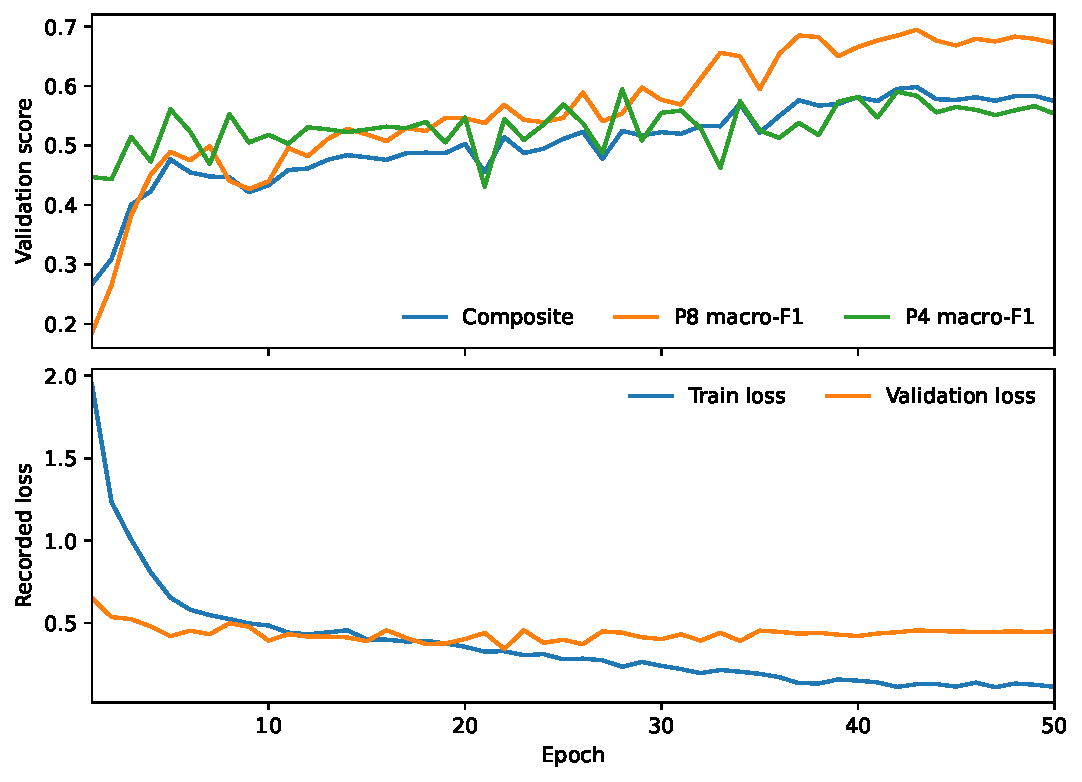
\includegraphics[width=.9\linewidth]{fig16768_internal_history}
\caption{Internal training and validation trajectories printed by job 16768. Values retain the precision of the epoch log; the final report retains more digits. These are not performance estimates for released specialists.\label{fig:trajectory}}
\end{figure}


\begin{table}[htbp]
\caption{Archived V3F internal summary. Values are from the last of eight epochs.\label{tab:app_pathology_ft}}
\centering\small
\begin{tabular}{lr}
\toprule
Recorded field & Value \\
\midrule
Rhythm validation windows & 144 \\
Pathology validation windows & 776 \\
Rhythm macro-F1 & 0.751823 \\
Rhythm top-1 & 0.708333 \\
P4 macro-F1 & 0.518821 \\
\bottomrule
\end{tabular}
\end{table}

\begin{table}[htbp]
\caption{Archived internal P4 calibration observations and cutoffs.\label{tab:app_path_spec}}
\centering\small
\begin{tabular}{lrrrr}
\toprule
Panel & Windows & Cutoff & Internal accuracy & Internal F1 \\
\midrule
ASMI & 432 & 0.67 & 0.794 & 0.7813 \\
LVH & 374 & 0.705 & 0.7487 & 0.7513 \\
IMI & 492 & 0.635 & 0.7927 & 0.8075 \\
ISC\_ & 194 & 0.595 & 0.8814 & 0.8856 \\
\bottomrule
\end{tabular}
\end{table}

\begin{table}[htbp]
\caption{Nine retained V3C candidates; selection by stable-tail rank, not peak.\label{tab:app_optuna_trials}}
\centering\small
\begin{tabular}{lrr}
\toprule
Trial & Ranking score & Peak composite \\
\midrule
0 & 0.5877250171 & 0.6087009381 \\
1 & 0.5637407072 & 0.5884071929 \\
2 & 0.5858734322 & 0.6483309166 \\
3 & 0.5996263228 & 0.6139392727 \\
4 & 0.5820539109 & 0.6472270611 \\
5 & 0.5822570086 & 0.5923444733 \\
6 & 0.6245117257 & 0.6313837131 \\
7 & 0.5635969384 & 0.6402737567 \\
8 & 0.5831962899 & 0.6509403856 \\
\bottomrule
\end{tabular}
\end{table}

\begin{table}[tbp]
\caption{P6 selected ECGs by retained source family. Wilson intervals use ECGs, not patients.\label{tab:app_source_primary6}}
\centering\small
\begin{tabular}{lrrrr}
\toprule
Source family & ECGs & Correct & Top-1 & Wilson 95\% CI \\
\midrule
chapman\_shaoxing & 1514 & 1447 & 95.57\% & 94.42\% to 96.50\% \\
codetest & 19 & 16 & 84.21\% & 62.43\% to 94.48\% \\
data\_test & 63 & 61 & 96.83\% & 89.14\% to 99.13\% \\
training/cpsc\_2018 & 5 & 5 & 100.00\% & 56.55\% to 100.00\% \\
training/cpsc\_2018\_extra & 8 & 6 & 75.00\% & 40.93\% to 92.85\% \\
training/georgia & 6 & 5 & 83.33\% & 43.65\% to 96.99\% \\
training/ningbo & 10 & 8 & 80.00\% & 49.02\% to 94.33\% \\
training/ptb-xl & 18 & 16 & 88.89\% & 67.20\% to 96.90\% \\
\bottomrule
\end{tabular}
\end{table}

\begin{table}[tbp]
\caption{P4 retained source alias. Pooled observation accuracy is not the mean of the four panel accuracies.\label{tab:app_source_primary4}}
\centering\small
\begin{tabular}{lrrr}
\toprule
Source alias & Observations & Correct & Pooled accuracy \\
\midrule
PTBXL\_FULL\_100HZ\_DERIVED & 962 & 776 & 80.67\% \\
\bottomrule
\end{tabular}
\end{table}

\begin{table}[htbp]
\caption{Scope of routing evidence. Historical June entries are not estimable.\label{tab:app_quarantine_transitions}}
\centering\small
\begin{tabular}{lrr}
\toprule
Analysis & Unit & Outcome \\
\midrule
June historical quarantine & ECG & Not estimable \\
SPH later joint policy & ECG & 2,478/12,869 withheld \\
LUDB later P6 fallback & ECG & 48/48 routed to P6 \\
LUDB unresolved after fallback & Known opportunities & 77/924 \\
\bottomrule
\end{tabular}
\end{table}

\begin{table}[tbp]
\caption{P8 statement-level decisions at the released thresholds. Positives are reference statements.\label{tab:p8class}}
\centering\small
\begin{tabular}{lrrrrrrr}
\toprule
Class & Positive & Total & Precision & Recall & Specificity & F1 & Cutoff \\
\midrule
AFIB & 390 & 2193 & 92.91\% & 90.77\% & 98.50\% & 91.83\% & 0.800 \\
SB & 792 & 2193 & 94.20\% & 94.32\% & 96.72\% & 94.26\% & 0.550 \\
STACH & 362 & 2193 & 91.53\% & 89.50\% & 98.36\% & 90.50\% & 0.800 \\
NSR & 592 & 2193 & 88.30\% & 79.05\% & 96.13\% & 83.42\% & 0.525 \\
RBBB & 116 & 2193 & 74.60\% & 81.03\% & 98.46\% & 77.69\% & 0.725 \\
PAC & 103 & 2193 & 47.52\% & 46.60\% & 97.46\% & 47.06\% & 0.450 \\
1AVB & 80 & 2193 & 68.66\% & 57.50\% & 99.01\% & 62.59\% & 0.775 \\
PVC & 94 & 2193 & 65.48\% & 58.51\% & 98.62\% & 61.80\% & 0.725 \\
\bottomrule
\end{tabular}
\end{table}

\begin{table}[htbp]
\caption{Minimum fields used to recalculate archived selected results.\label{tab:app_record_schema}}
\centering\small
\begin{tabular}{@{}p{.29\linewidth}p{.64\linewidth}@{}}
\toprule
Field & Use \\
\midrule
ECG identifier & Links observations within the retained analysis \\
Source alias & Defines a retained source stratum, not patient independence \\
Reference and score & Defines binary ROC and decision comparison \\
Top-1 and accepted set & Defines rhythm correctness \\
Endpoint and binary decision & Defines pathology panel counts \\
\bottomrule
\end{tabular}
\end{table}


To verify a published file, download it from release v0.1.0 and run
\path{sha256sum FILE} or \path{Get-FileHash -Algorithm SHA256 FILE}. Compare the full digest and byte length in Table~\ref{tab:app_hashes}. V3F and V3AG are distinct waveform backbones; V3P and V3Q are P6 and P8 specialist weights; the remaining V3AG file is the P4 specialist. The unrecovered historical Optuna database and the generic predictions file formerly listed are not represented as verified release objects.
\begin{table}[tbp]
\caption{Verified release v0.1.0 artifacts. Linked filenames download the specific artifacts. Each digest covers the named file only.\label{tab:app_hashes}}
\centering\small
\begin{tabular}{@{}p{.33\linewidth}rp{.45\linewidth}@{}}
\toprule
File & Bytes & SHA-256 \\
\midrule
\href{https://github.com/Mateo197802/titan-v45-ecg-multihead/releases/download/v0.1.0/backbone-v3f-original.pt}{\nolinkurl{backbone-v3f-original.pt}} & 233,565,900 & \texttt{ca5d4dcb4b9828e6c4339800fe81ec27}\newline\texttt{f32d9b09a090bb57503bfb56746a8da8} \\
\href{https://github.com/Mateo197802/titan-v45-ecg-multihead/releases/download/v0.1.0/specialists-v3p-e008-primary6-diagnostic.pt}{\nolinkurl{specialists-v3p-e008-primary6-diagnostic.pt}} & 22,354,966 & \texttt{9c5a9265a7155e1206c551cc4e6d645b}\newline\texttt{86363ba3dbdeb7baf7b9f173c314be3d} \\
\href{https://github.com/Mateo197802/titan-v45-ecg-multihead/releases/download/v0.1.0/specialists-v3q-primary8-best-candidate.pt}{\nolinkurl{specialists-v3q-primary8-best-candidate.pt}} & 29,498,326 & \texttt{b30cb2bbb45f1231c93ff1c196aa966b}\newline\texttt{57b49831cadb296131c0283e7b0ceb02} \\
\href{https://github.com/Mateo197802/titan-v45-ecg-multihead/releases/download/v0.1.0/backbone-v3ag-pathology.pt}{\nolinkurl{backbone-v3ag-pathology.pt}} & 233,566,092 & \texttt{bf71e4cf8acc34031cb3611c7031e064}\newline\texttt{9822e705fd7dcea354a3ea583ce920ee} \\
\href{https://github.com/Mateo197802/titan-v45-ecg-multihead/releases/download/v0.1.0/specialists-v3ag-primary4-calibrated.pt}{\nolinkurl{specialists-v3ag-primary4-calibrated.pt}} & 29,413,606 & \texttt{cf5091e962fffb3254b1a71fe57236dd}\newline\texttt{82ea0139093df192511499d931391dbc} \\
\bottomrule
\end{tabular}
\end{table}


\reftitle{References}
\begin{thebibliography}{999}
\bibitem[Reyna et~al.(2022)]{Reyna2022Challenge}
Reyna, M.A.; et al. Issues in the automated classification of multilead ECGs using heterogeneous labels and populations. \emph{Physiol. Meas.} \textbf{2022}, 43, 084001. doi:10.1088/1361-6579/ac79fd.
\bibitem[Wagner et~al.(2020)]{Wagner2020PTBXL}
Wagner, P.; et al. PTB-XL, a large publicly available electrocardiography dataset. \emph{Sci. Data} \textbf{2020}, 7, 154. doi:10.1038/s41597-020-0495-6.
\bibitem[Rossi et~al.(2026)]{Rossi2026AF}
Rossi, M.; et al. Clinical characteristics and outcomes of first diagnosed atrial fibrillation: Insights from 2 prospective registries in Europe and Asia. \emph{Heart Rhythm} \textbf{2026}, 23, 356--367. doi:10.1016/j.hrthm.2025.08.007.
\bibitem[Hannun et~al.(2019)]{Hannun2019Cardiologist}
Hannun, A.Y.; Rajpurkar, P.; Haghpanahi, M.; Tison, G.H.; Bourn, C.; Turakhia, M.P.; Ng, A.Y.
\newblock Cardiologist-level arrhythmia detection and classification in ambulatory electrocardiograms using a deep neural network.
\newblock {\em Nat. Med.} {\bf 2019}, {\em 25},~65--69. \url{https://doi.org/10.1038/s41591-018-0268-3}.

\bibitem[Ribeiro et~al.(2020)]{Ribeiro2020Automatic}
Ribeiro, A.H.; Ribeiro, M.H.; Paix{\~a}o, G.M.M.; Oliveira, D.M.; Gomes, P.R.; Canazart, J.A.; Ferreira, M.P.S.; Andersson, C.R.; Macfarlane, P.W.; Meira~Jr, W.; Sch{\"o}n, T.B.; Ribeiro, A.L.P.
\newblock Automatic diagnosis of the 12-lead ECG using a deep neural network.
\newblock {\em Nat. Commun.} {\bf 2020}, {\em 11},~1760. \url{https://doi.org/10.1038/s41467-020-15432-4}.

\bibitem[Zhu et~al.(2020)]{Zhu2020Automatic}
Zhu, H.; Cheng, C.; Yin, H.; Li, X.; Zuo, P.; Ding, J.; Lin, F.; Wang, J.; Zhou, B.; Bi, X.; et~al.
\newblock Automatic multilabel electrocardiogram abnormal findings detection using a deep convolutional neural network.
\newblock {\em Comput. Biol. Med.} {\bf 2020}, {\em 125},~103986. \url{https://doi.org/10.1016/j.compbiomed.2020.103986}.

\bibitem[Strodthoff et~al.(2021)]{Strodthoff2021Deep}
Strodthoff, N.; Wagner, P.; Schaeffter, T.; Samek, W.
\newblock Deep Learning for ECG Analysis: Benchmarks and Insights from PTB-XL.
\newblock {\em IEEE J. Biomed. Health Inform.} {\bf 2021}, {\em 25},~1519--1528. \url{https://doi.org/10.1109/JBHI.2020.3022989}.

\bibitem[Vranken et~al.(2021)]{Vranken2021Uncertainty}
Vranken, J.F.; van de Leur, R.R.; et al. Uncertainty estimation for deep learning-based automated analysis of 12-lead electrocardiograms. \emph{Eur. Heart J. Digit. Health} \textbf{2021}, 2, 401--415. doi:10.1093/ehjdh/ztab045.


\bibitem[Mastoi et~al.(2022)]{Mastoi2022DERMA}
Mastoi, Q.; Wah, T.Y.; et al. Novel DERMA Fusion Technique for ECG Heartbeat Classification. \emph{Life} \textbf{2022}, 12, 842. doi:10.3390/life12060842.


\bibitem[Herman et~al.(2024)]{Herman2024}
Herman, R.; Demolder, A.; et al. Validation of an automated artificial intelligence system for 12-lead ECG interpretation. \emph{J. Electrocardiol.} \textbf{2024}, 82, 147--154. doi:10.1016/j.jelectrocard.2023.12.009.




\bibitem[Elsheikhy et~al.(2025)]{Elsheikhy2025Lightweight}
Elsheikhy, D.H.; Hassan, A.S.; Yhiea, N.M.; Fareed, A.M.; Rashed, E.A. Lightweight Deep Learning Architecture for Multi-Lead ECG Arrhythmia Detection. \emph{Sensors} \textbf{2025}, 25, 5542. doi:10.3390/s25175542.


\bibitem[Zhou et~al.(2025)]{Zhou2025Classification}
Zhou, F.; Fang, D. Classification of multi-lead ECG based on multiple scales and hierarchical feature convolutional neural networks. \emph{Sci. Rep.} \textbf{2025}, 15, 16418. doi:10.1038/s41598-025-94127-6.



\bibitem[Li et~al.(2024)]{Li2024DualView}
Li, H.; Han, J.; Zhang, H.; Zhang, X.; Si, Y.; Zhang, Y.; Liu, Y.; Yang, H.
Clinical knowledge-based ECG abnormalities detection using dual-view CNN-Transformer and external attention mechanism.
\emph{Comput. Biol. Med.} \textbf{2024}, 178, 108751. doi:10.1016/j.compbiomed.2024.108751.

\bibitem[He et~al.(2016)]{He2016Deep}
He, K.; Zhang, X.; Ren, S.; Sun, J.
\newblock Deep Residual Learning for Image Recognition.
\newblock In Proceedings of the IEEE Conference on Computer Vision and Pattern Recognition (CVPR), Las Vegas, NV, USA, 27--30 June 2016; pp. 770--778.

\bibitem[Hu et~al.(2018)]{Hu2018Squeeze}
Hu, J.; Shen, L.; Sun, G.
\newblock Squeeze-and-Excitation Networks.
\newblock In Proceedings of the IEEE Conference on Computer Vision and Pattern Recognition (CVPR), Salt Lake City, UT, USA, 18--23 June 2018; pp. 7132--7141.

\bibitem[Vaswani et~al.(2017)]{Vaswani2017Attention}
Vaswani, A.; Shazeer, N.; Parmar, N.; Uszkoreit, J.; Jones, L.; Gomez, A.N.; Kaiser, L.; Polosukhin, I.
\newblock Attention Is All You Need.
\newblock In Advances in Neural Information Processing Systems (NeurIPS); Long Beach, CA, USA, 4--9 December 2017; Vol.~30, pp. 5998--6008.

\bibitem[Lin et~al.(2017)]{Lin2017Focal}
Lin, T.Y.; Goyal, P.; Girshick, R.; He, K.; Doll{\'a}r, P.
\newblock Focal Loss for Dense Object Detection.
\newblock In Proceedings of the IEEE International Conference on Computer Vision (ICCV), Venice, Italy, 22--29 October 2017; pp. 2980--2988.

\bibitem[Akiba et~al.(2019)]{Akiba2019Optuna}
Akiba, T.; Sano, S.; Yanase, T.; Ohta, T.; Koyama, M.
\newblock Optuna: A Next-generation Hyperparameter Optimization Framework.
\newblock In Proceedings of the 25th ACM SIGKDD International Conference on Knowledge Discovery and Data Mining (KDD), Anchorage, AK, USA, 4--8 August 2019; pp. 2623--2631.

\bibitem[Szegedy et~al.(2016)]{Szegedy2016Rethinking}
Szegedy, C.; Vanhoucke, V.; Ioffe, S.; Shlens, J.; Wojna, Z.
\newblock Rethinking the Inception Architecture for Computer Vision.
\newblock In Proceedings of the IEEE Conference on Computer Vision and Pattern Recognition (CVPR), Las Vegas, NV, USA, 27--30 June 2016; pp. 2818--2826.

\bibitem[Pan and Tompkins(1985)]{Pan1985Real}
Pan, J.; Tompkins, W.J.
\newblock A Real-Time QRS Detection Algorithm.
\newblock {\em IEEE Trans. Biomed. Eng.} {\bf 1985}, {\em BME-32},~230--236. \url{https://doi.org/10.1109/TBME.1985.325532}.

\bibitem[Selvaraju et~al.(2017)]{Selvaraju2017Grad}
Selvaraju, R.R.; Cogswell, M.; Das, A.; Vedaldi, A.; Parikh, D.; Batra, D.
\newblock Grad-CAM: Visual Explanations from Deep Networks via Gradient-Based Localization.
\newblock In Proceedings of the IEEE International Conference on Computer Vision (ICCV), Venice, Italy, 22--29 October 2017; pp. 618--626.

\bibitem[Wilson(1927)]{Wilson1927Probable}
Wilson, E.B.
\newblock Probable Inference, the Law of Succession, and Statistical Inference.
\newblock {\em J. Am. Stat. Assoc.} {\bf 1927}, {\em 22},~209--212.

\bibitem[Efron(1979)]{Efron1979Bootstrap}
Efron, B.
\newblock Bootstrap Methods: Another Look at the Jackknife.
\newblock {\em Ann. Stat.} {\bf 1979}, {\em 7},~1--26.

\bibitem[Hanley and McNeil(1982)]{Hanley1982meaning}
Hanley, J.A.; McNeil, B.J.
\newblock The meaning and use of the area under a receiver operating characteristic (ROC) curve.
\newblock {\em Radiology} {\bf 1982}, {\em 143},~29--36.
\end{thebibliography}

\end{document}
